% ---------------------------------------------------------------------------------------------------------------
% TEMPLATE PARA TRABALHO DE CONCLUSÃO DE CURSO
% Idealizado por Sérgio Custódio e Kelvin Pinheiro
% Adaptador por Raphael de Souza Nunes (Universidade do Estado do Amazonas)
% Baseado no projeto: http://tcc.tsi.gp.utfpr.edu.br/paginas/modelos-latex-da-utfpr
% De:         Diego Marczal e 
% 	          Michael Vornes
% Universidade Federal do Pará - Faculdade de Engenharia Mecânica
% ---------------------------------------------------------------------------------------------------------------

% CARREGA CLASSE PERSONALIZADA DA FEM/UFPA--------------------------------------------------------------------------
\documentclass[%twoside,                   % Impressão em frente e verso
oneside,                                   % Impressão apenas frente
]{ufpa-fem-abntex2}

\usepackage{enumerate}

%INCLUI ARQUIVOS DO TRABALHO DE CONCLUSÃO DE CURSO (PRÉ-TEXTUAIS, TEXTUAIS, PÓS-TEXTUAIS)-----------------------
%%%%%

% INSERE CAPA E FOLHA DE ROSTO
% CAPA-------------------------------------------------------------------

% ORIENTAÇÕES GERAIS-------------------------------------------------------------------------------------
% Caso algum dos campos não se aplique ao seu trabalho, como por exemplo,
% se não houve coorientador, apenas deixe vazio.
% Exemplos: 
% \coorientador{}
% \departamento{}

% DADOS DO TRABALHO--------------------------------------------------------------------------------------
\titulo{\textbf{Projeto de um sistema de abastecimento pluvial baseado em \textit{iot}}}
\subtitulo{} %Se não hover subtítulo, deixar em branco.
\titleabstract{Title in English}
\autor{Raphael de Souza Nunes}
\autorcitacao{NUNES, Raphael} % Sobrenome em maiúsculo
\local{Manaus/AM}
\data{2021}

% NATUREZA DO TRABALHO-----------------------------------------------------------------------------------
\projeto{Trabalho de Conclusão de Curso}

% TÍTULO ACADÊMICO---------------------------------------------------------------------------------------
\tituloAcademico{Bacharel}

% ÁREA DE CONCENTRAÇÃO E LINHA DE PESQUISA---------------------------------------------------------------
% Se a natureza for Trabalho de Conclusão de Curso, deixe ambos os campos vazios
% Se for programa de Pós-graduação, indique a área de concentração e a linha de pesquisa
\areaconcentracao{}
\linhapesquisa{}

% DADOS DA INSTITUIÇÃO-----------------------------------------------------------------------------------
% Se a natureza for Trabalho de Conclusão de Curso, coloque o nome do curso de graduação em "programa"
% Formato para o logo da Instituição: \logoinstituicao{<escala>}{<caminho/nome do arquivo>}
\instituicao{Universidade do Estado do Amazonas}
\departamento{Escola Superior de Tecnologia}
\programa{Graduação em Engenharia de Controle e Automação}
\logoinstituicao{14cm}{figuras/institucional/brasao_capa.jpg} %

% DADOS DOS ORIENTADORES---------------------------------------------------------------------------------
\orientador{\textbf{Prof. Dr. Israel Mazaira Morales}}
%\orientador[Orientadora:]{Nome da orientadora}
\instOrientador{Universidade do Estado do Amazonas}

%\coorientador{Nome do coorientador}
%\coorientador[Coorientadora:]{Nome da coorientadora}
%\instCoorientador{Instituição do coorientador}

% FOLHA DE ROSTO-------------------------------------------------------------------

% Este arquivo não precisa ser alterado

%% TRABALHO DE CONCLUSÃO DE CURSO
\preambulo{{\imprimirprojeto} apresentado à banca avaliadora do curso de Engenharia de Controle e Automação da {\imprimirinstituicao} - UEA, unidade Escola Superior de Tecnologia - EST, como pré-requisito para obtenção do título de {\imprimirtituloAcademico} em Engenharia de Controle e Automação.}
% ---
% Inserir folha de aprovação
% ---
% Isto é um exemplo de Folha de aprovação, elemento obrigatório da NBR
% 14724/2011 (seção 4.2.1.3). Você pode utilizar este modelo até a aprovação do trabalho. Após isso, substitua todo o conteúdo deste arquivo por uma imagem da página assinada pela banca com o comando abaixo:
%
% \includepdf{folhadeaprovacao_final.pdf}
%


\dataaprovacao{10/10/2020}
\conceito{} %Antes da defesa, não adicionar valor ao compo. Após a defesa, pode-se adicionar Regular, Bom ou Excelente e solicitar as assinaturas da banca examinadora.
 
\nomePrimeiromembro{Prof. Esp. Sérgio de Souza Custódio Filho}
\instPrimeiromembro{FEM/ITEC/UFPA}
 
\nomeSegundomembro{Prof. Me. Fábio Antônio do Nascimento Setúbal}
\instSegundomembro{FEM/ITEC/UFPA}

%Ocultar ou não dependendo do numero de professores na banca. Ver arquivo de configuracao \assinatura{\imprimirnomeTerceiromembro  \\ Membro - \imprimirinstTerceiromembro}  nas configuracoes ufpa-fem-abntex2.cls.

%\nomeTerceiromembro{Eng. Beltrano Cunha} 
%\instTerceiromembro{Externo (PETROBRAS)}

%ª
 


\begin{document}
	
	\pretextual
	\imprimircapa                                  
	\imprimirfolhaderosto{}                           
	%\imprimirfolhadeaprovacao{}
	%% DEDICATÓRIA------------------------------------------------------------------

\renewcommand{\dedicatorianame}{DEDICATÓRIA}

\begin{dedicatoria}

Dedico aos meus pais e a toda a minha família.

\end{dedicatoria}
        
	%% AGRADECIMENTOS---------------------------------------------------------------

\begin{agradecimentos}[AGRADECIMENTOS]

Agradeço a Deus pelo dom da vida e do conhecimento os quais me proporcionaram chegar até aqui.

Agradeço a minha família por todo apoio, paciência e dedicação contribuindo diretamente para que eu pudesse traçar o meu caminho de forma mais fácil durante todos esses anos.

Agradeço aos meus pais, Wagner Antônio da Silva Nunes e Mariluce de Souza Nunes, que sempre me incentivam e me guiaram pelos meus caminhos do conhecimento.

Agradeço todos os meus professores da Universidade do Estado do Amazonas, em especial, os professores: Israel Mazaira, Moisés Bastos, Charles Melo, Jozias Parente, Raimundo Cláudio, Israel Torné e Fábio Cardoso os quais não mediram esforços para transmitir o conhecimento sejam eles em sala de aula, em projetos ou mesmo em conversas pelos corredores da universidade.

Agradeço o apoio de todos os meus amigos da universidade, em especial, Michael Sidi, Mateus Ramos, Samuel Marinho, Rubens Andrade e Isaque Vilson.

Por último, quero agradecer também à Universidade do Estado do Amazonas e todo o seu corpo docente.


\end{agradecimentos}

	%% EPÍGRAFE---------------------------------------------------------------------

\renewcommand{\epigraphname}{EPÍGRAFE}

\begin{epigrafe}

\textit{``A matemática é o alfabeto no qual Deus escreveu o universo.'' (Galileu Galilei)}

\end{epigrafe}

% OBSERVAÇÕES------------------------------------------------------------------
% Altere o texto para inserir a epígrafe do seu trabalho


	% RESUMO--------------------------------------------------------------------------------

\begin{resumo}[RESUMO]
\begin{SingleSpacing}

 Com base na busca da produção de tecnologias para diminuir a degradação do meio ambiente e, unindo-se a isto, a procura pela implementação de \textit{Smart Things}, dentro do âmbito do \textit{IoT - Internet Of Things},  o projeto a ser desenvolvido visa a elaboração de um protótipo de uma \textbf{Cisterna Automatizada - CA} a qual contará com um sistema físico para coleta e distribuição de água da chuva, integrando as três áreas de um projeto \textit{IoT}: \textit{Hardware}, \textit{Firmware} e \textit{Software}. No segmento de \textit{Firmware}, por meio do uso de microcontroladores e microprocessadores em integração com sensores, atuadores e a \textit{Intranet}, será possível coletar dados e realizar ações pré-estabelecidas ou em tempo real oriundas de comandos do usuário, assim como receber atualizações para melhoria contínua do Software Embarcado (\textit{Firmware Update}).  Na seção de \textit{Software}, a utilização de tecnologias para modelagem de aplicações \textit{Mobile} e \textit{Desktop}, como  \textit{React Native} e \textit{Electron},  garantiram a criação de interfaces amigáveis para rotinas de cadastro, atualização, monitoramento e controle dos processos do sistema de coleta. Por fim, no campo de \textit{Hardware}, houve a implementação dos esquemáticos e \textit{layout's 3D}  para fabricação das placas de circuito impresso - PCB's. Com intuito de validação, um protótipo foi construído contendo estruturas de: alimentação, conversão de sinais, comunicação, controle e acionamento além do desenho peças estruturais, para serem implementadas posteriormente com base em manufatura aditiva.
 
\vspace{\onelineskip}

\textbf{Palavras-chave}: \textit{IoT - Internet of Things}. \textit{Smart Things}. \textit{Intranet}.  Cisterna Inteligente. \textit{Firmware}. \textit{Hardware}. \textit{Software}. \textit{React Native}. \textit{Electron.js}.

\end{SingleSpacing}
\end{resumo}

% OBSERVAÇÕES---------------------------------------------------------------------------
% Altere o texto inserindo o Resumo do seu trabalho.
% Escolha de 3 a 5 palavras ou termos que descrevam bem o seu trabalho .
% As palavras-chave são separadas por pontos. Apenas a primeira letra é maiúscula.

 % Resumo em Português
	%% ABSTRACT--------------------------------------------------------------------------------

\begin{resumo}[ABSTRACT]
\begin{SingleSpacing}


Based on the search for the production of technologies to reduce the degradation of the environment and, joining this, the trend towards the implementation of Smart Things, within the scope of the IoT - Internet Of Things, the developed project aimed at the development of a system to create an Automated Cistern which has a physical prototype for simulating the collection and distribution of rainwater, integrating the three areas of an IoT project: Hardware, Firmware and Software. In the Firmware segment, through the use of microcontrollers and microprocessors in integration with sensors, actuators and the Intranet, it will be possible to collect data and perform pre-established or real-time actions from user commands, as well as receive updates for continuous improvement of the Embedded Software (Firmware Update). In the Software section, the use of technologies for modeling Mobile and Desktop applications, such as React Native and Electron, ensured the creation of friendly interfaces for routines for registration, updating, monitoring and control of the collection system processes. Finally, in the field of Hardware, 3D schematics and layouts were developed for the manufacture of printed circuit boards - PCB's. With the purpose of validation, the built prototype has structures for: power, signal conversion, communication, control and activation. For local application, drawings of structural parts were also developed, to be made later based on additive manufacturing.

\vspace{\onelineskip}

\textbf{Keywords}: \textit{IoT - Internet of Things}. \textit{Smart Things}. \textit{Intranet}.   \textit{Firmware}. \textit{Hardware}. \textit{Software}. \textit{React Native}. \textit{Electron}.

\end{SingleSpacing}
\end{resumo}

% OBSERVAÇÕES---------------------------------------------------------------------------
% Altere o texto inserindo o Abstract do seu trabalho.
% Escolha de 3 a 5 palavras ou termos que descrevam bem o seu trabalho 
% As palavras-chave são separadas por pontos. Apenas a primeira letra é maiúscula. % Resumo em Inglês
	% Lista de Figuras----------------------------------------------------------------

\pdfbookmark[0]{\listfigurename}{lof}
\listoffigures*
\cleardoublepage

% OBSERVAÇÕES---------------------------------------------------------------------
% Este arquivo não precisa de ser alterado, pois a lista é gerada automaticamente.

	%% LISTA DE QUADROS----------------------------------------------------------------

\renewcommand{\listofquadrosname}{LISTA DE QUADROS}

\pdfbookmark[0]{\listofquadrosname}{loq}
\listofquadros*
\cleardoublepage

% OBSERVAÇÕES---------------------------------------------------------------------
% Este arquivo não necessita de ser editado. A lista é gerada automaticamente.

	%% LISTA DE TABELAS-------------------------------------------------------------

\pdfbookmark[0]{\listtablename}{lot}
\listoftables*
\cleardoublepage

% OBSERVAÇÕES-------------------------------------------------------------------
% Este arquivo não precisa ser alterado, pois a lista é gerada automaticamente.
 % Lista de Tabelas
	% LISTA DE ABREVIATURAS E SIGLAS----------------------------------------------------------

\begin{siglas}
    \item[IoT] Internet Of Things
    \item[PCB] Printed Circuit Board
    \item[SMCC] Sistema de Medição e Controle da Cisterna
    \item[SMCCD] Sistema de Medição e Controle da Caixa D'água
    \item[MQTT]  Message Queuing Telemetry Transport
    \item[HTTP] Hypertext Transfer Protocol
    \item[GPIO] General Purpose Input Output
    \item[HAS] Home Automation System
    \item[DC] Direct Current
    \item[AC] Alternate Current
    \item[PWM] Pulse-Width Modulation
    \item[NF] Normalmente Fechada
    \item[IDE]  Integrated Development Environment
    \item[CLI] Command Line Interface
    \item[GUI] Graphic User Interface
    \item [HTML] HyperText Markup Language
    \item[CSS] Cascading Style Sheet
\end{siglas}

% OBSERVAÇÕES-----------------------------------------------------------------------------
% Altere a lista acima para definir os acrônimos e siglas utilizados neste trabalho
          		%% LISTA DE SÍMBOLOS------------------------------------------------------------

\begin{simbolos}
    \item[$ \Gamma $] Letra grega Gama
    \item[$ \lambda $] Comprimento de onda
    \item[$ \in $] Pertence ...
\end{simbolos}

% OBSERVAÇÕES-------------------------------------------------------------------
% Altere a lista acima para definir os símbolos utilizados no trabalho

	%% LISTA DE ALGORITMOS----------------------------------------------------------

\newcommand{\algoritmoname}{Algoritmo}
\renewcommand{\listalgorithmcfname}{LISTA DE ALGORITMOS}

\floatname{algocf}{\algoritmoname}
\newlistof{listofalgoritmos}{loa}{\listalgoritmoname}
\newlistentry{algocf}{loa}{0}

\counterwithout{algocf}{chapter}
\renewcommand{\cftalgocfname}{\algoritmoname\space}
\renewcommand*{\cftalgocfaftersnum}{\hfill--\hfill}

\pdfbookmark[0]{\listalgorithmcfname}{loa}
\listofalgorithms
\cleardoublepage

% OBSERVAÇÕES------------------------------------------------------------------
% Este arquivo não precisa ser alterado, pois a lista é gerada automaticamente.

	% SUMÁRIO----------------------------------------------------------------------

\renewcommand{\contentsname}{SUMÁRIO}

\pdfbookmark[0]{\contentsname}{toc}
\tableofcontents*
\cleardoublepage

% OBSERVAÇÕES-------------------------------------------------------------------
% Este arquivo não precisa ser alterado, pois o sumário é gerado automaticamente.
               			   
	%Verificar folha de Aprovação e Catalogação Bibliográfica
	
	% Sumário
	
	\textual
	% INSERE ELEMENTOS TEXTUAIS
	% INTRODUÇÃO-------------------------------------------------------------------

\chapter{INTRODUÇÃO}
\label{chap:introducao}


A água é um recurso básico para a sustentação humana em um ambiente e ao longo do tempo várias civilizações evoluíram e padeceram em função de sua relação de uso com este recurso. Nos últimos anos, crises relacionadas ao abastecimento e à qualidade da água potável têm sido observadas em todo o Globo. Tomando o Brasil como exemplo, percebe-se uma distribuição desigual: No norte do pais há grandes reservas de água, porém nas regiões Nordeste e Sudeste há problemas de escassez e poluição dos rios.


A região norte, possuindo a maior reserva de água potável do Brasil e também os maiores índices de precipitação, é a região que possui as taxas mais altas de desperdício \cite{globo}. O desperdício pode ser encontrado no ambiente doméstico e nas várias etapas de: coleta, armazenamento, processamento e principalmente na distribuição do recurso. 

A instalação de uma cisterna garante, pelo menos, três pontos positivos: que seja possível utilizar a água de precipitações para afazeres domésticos, reduzindo o consumo mensal de determinada residência; pode diminuir o desperdício durante a etapa de distribuição da concessionária e contribuir para a redução da
incidência de inundações em grandes cidades, uma vez que grande parte dessa água não seria descartada, mas armazenada.

A aplicação de uma cisterna automatizada garante uma supervisão do nível de água constantemente assim como o controle/acionamento de bombas para alimentação de tanques ou caixas d’agua para tarefas específicas trazendo comodidade e fomentando os motivos de aplicação.
	% PROBLEMÁTICA-------------------------------------------------------------------

\chapter{PROBLEMÁTICA}
\label{chap:problematica}

Segundo a Gartner, Inc BizMeet desde 2017 existem mais objetos conectados à Internet do que as 7 bilhões de pessoas no mundo. Isso demonstra uma crescente busca pela obtenção e controle das mais diversas tarefas. Os objetos e dispositivos estão adquirindo funcionalidades as quais se identificam com os ramos da \textit{IoT}, tornando-se possível a concepção de diversas melhorias no funcionamento, através da obtenção e distribuição de dados.  A utilização da \textbf{Internet das Coisas} está tão conectada ao nosso cotidiano que ocasiona o nascimento de tecnologias necessariamente conectadas, como \textit{Smart Home} e \textit{Smart Buildings}. 

Diante disso, em ambientes como na região Amazônica, onde há altos índices de precipitação, a implantação de cisternas para utilização da água da chuva se torna bastante viável. Sabe-se que a água da chuva não é própria para o consumo e para o preparo de alimentos, porém a mesma pode ser utilizada em afazeres como limpeza de locais e também em descargas de banheiros, onde há o maior nível de desperdício.

Em virtude do que foi mencionado,  a aplicação de uma cisterna se torna algo viável para a economia de água ajudando na conservação do meio ambiente, porém, a automação do processo de coleta e distribuição trará reais vantagens quando comparada à um processo manual? Quais serão os problemas recorrentes ao se implementar tal sistema?  Será possível uma aplicação em diversos contextos e localidades?  O auxílio de tecnologias como o \textit{WIFI} unido à \textit{IoT} fará com que a aplicação seja mais vantajosa?  A utilização da água coletada por meio de uma cisterna automatizada, onde haverá gastos, como consumo energia elétrica, aplicação de sensoriamento, motobombas, sistemas hidráulicos, entre outros, trará benefícios financeiros quando comparado à utilização de água através, unicamente, da rede tradicional?

	% OBJETIVOS-------------------------------------------------------------------

\chapter{OBJETIVOS}
\label{chap:objetivos}

\section{Objetivo geral}
\label{sec:objetivogeral}
O objetivo desse trabalho de conclusão de curso é a elaboração de um projeto base para aplicação de um sistema automatizado de coleta, armazenamento e distribuição de água da chuva com base em uma cisterna pluvial. Realizando medições de volume, através de sensores, acionamento de válvulas solenoides e motobombas por meio de comandos via interfaces \textit{desktop} e \textit{mobile}. A elaboração também contará com a criação de circuitos esquemáticos para desenvolvimento de placas de circuito impresso - \textit{PCB's}, o uso de microcontoladores e microprocessadores em conjunto com  diretrizes de Internet das Coisas - \textit{IoT},  assim como o uso de \textit{Frameworks} atuais baseados em \textit{Javascript} para criação de Interfaces Homem Máquina.

\section{Objetivos específicos}

\begin{description}
	\item [(a)] Elaborar um módulo denominado \textbf{CCM - \textit{Cistern Control Module}} para aplicação no reservatório principal, realizando medições de nível, acionamento de \textit{motobomba}, direcionamento do fluxo de água em conexão com outros dispositivos via tecnologia \textit{Wi-Fi}.
	\item [(b)] Elaborar um módulo denominado \textbf{TCM - \textit{Tank Control Module}} para aplicação no reservatório auxiliar, realizando medições de nível, direcionamento do fluxo de água em conexão com outros dispositivos via tecnologia \textit{Wi-Fi}.
	\item [(c)] Elaborar um aplicação \textit{Android Mobile} (denominada \textbf{RCS APP}) e \textit{Desktop} (denominada \textbf{RCS DESKTOP}) para executar as ações: ativação e desativação de uma bomba d'água, direcionamento do fluxo de água, visualização de dados provenientes de sensores e estruturando a possibilidade de definir as condições que executem rotinas de acionamento automático;
	\item [(d)] Configurar um sistema operacional embarcado conciso (baseado em \textit{kernel Linux}) aplicando-o a um microprocessador. O dispositivo deve possuir conexão com a \textit{Intranet} e servir como uma central de controle e armazenamento de dados, bem como ser hospedeiro do serviço de \textit{Broker MQTT};
	\item [(e)] Incluir no sistema, rotinas de leitura de sensores e acionamento de motobombas;
	\item [(f)] Organizar um repositório \textit{online} para realização de futuras atualizações (\textit{upgrades}) do \textit{firmware} embarcado.
\end{description}

\label{sec:objetivosespecificos}
	% HIPÓTESE E JUSTIFICATIVA-------------------------------------------------------------------

\chapter{HIPÓTESE E JUSTIFICATIVA}
\label{chap:hipoteseejustificativa}

\section{Hipótese}
\label{sec:hipotese}

A inclusão da \textit{IoT} nos mais diversos processos nos traz múltiplos benefícios, como: obter maiores informações e atuar sobre tais processos. Automatizar tarefas que são, muitas vezes repetitivas ou mesmo insalubres faz com que as tecnologias denominadas \textit{Smart} se tornem cada vez mais um foco de pesquisa e desenvolvimento. 

No âmbito do meio ambiente, a implantação de uma cisterna garante um menor desperdício de água, utilizando-a para tarefas específicas assim como uma economia no consumo. Porém a implantação de uma cisterna como não atrai indivíduos pois existe a necessidade de trabalho braçal assim como a constante análise da quantidade de água disponível.

Esse TCC busca elaborar uma cisterna autônoma trazendo benefícios, primeiramente financeiros,  e também ecológicos assim como benefícios da comodidade para a retirada e verificação dos níveis de água, tornando a ideia da aplicação mais atraente para possíveis clientes, em caso do projeto se tornar um produto. Com a redução significativa de consumo de água, será possível que o investimento de construção e aplicação retorne como economia.

\section{Justificativa}
\label{sec:justificativa}

Buscando estar de acordo com a convergência de produtos e processos conectados em rede, percebeu-se a necessidade e oportunidade da utilização de conceitos e tecnologias emergentes nos contextos atuais, como \textit{Smart Things}. A aplicação de serviços que unam a busca pela preservação ambiental e conceitos citados anteriormente se destacam por possibilitar uma gama de vantagens em qualquer processo.

O presente trabalho se justifica pelos altos índices de precipitação na região do Estado do Amazonas, onde será aplicado. A coleta de água da chuva acarretará, além da diminuição do consumo de água (trazendo economia para o usuário e ajudando na preservação ambiental), em uma distribuição mais inteligente da água não potável: que pode ser utilizada para limpezas, descargas e até irrigações; e em uma motivação para investimentos futuros reduzindo, ainda mais, os gastos de implementação.

O projeto trará motivações e investidores para aplicação de novas pesquisas focadas em contextos diferentes dentro do estado, onde há: \textbf{I}. lugares que não possuem estruturas de rede ou que demandam comunicação à grandes distâncias: utilização de tecnologias como \textit{LoRaWan}, \textit{SigFox} e \textit{Zigbee}; \textbf{II.} lugares que não possuem energia elétrica: união dos conceitos desse trabalho com fontes renováveis, como alimentação fotovoltaica.

	% TRABALHOS RELACIONADOS--------------------------------------------------------

\chapter{TRABALHOS RELACIONADOS}
\label{chap:trabalhosrelacionados}

\section{Automação e Controle em Sistema de Aproveitamento de Água da Chuva para 
Fins Não Potáveis}

\textbf{Autora:} Lilia Rodrigues Lucas Magalhães
\vspace{\onelineskip}

Este trabalho de conclusão de curso realizado por Lilia Rodrigues Lucas Magalhães pelo Centro Universitário de Brasília - UniCEUB apresenta uma protosta muito semelhante ao trabalho a ser desenvolvido.

A ideia deste projeto foi demonstrar o funcionamento automatizado de um sistema (representado na \autoref{fig:trab_rel_01} ) de aproveitamento de água de chuva por meio da elaboração de um protótipo composto pela maquete de um banheiro, confeccionada em madeira, juntamente com três reservatórios em acrílico. Esse cenário representa o sistema de distribuição de água de chuva dentro de uma residência e destina-se à utilização em descarga sanitária.

\begin{figure}[H]
	\centering
	\caption{Corte Esquemático do Sistema de Aproveitamento Proposto.}
	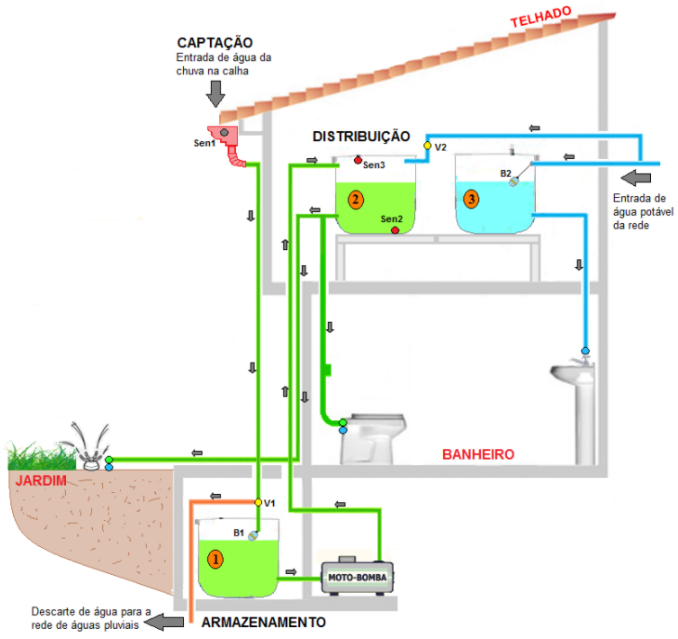
\includegraphics[width=0.7\textwidth]{figuras/trabalhos_relacionados/fig01.png}
	\label{fig:trab_rel_01}
\end{figure}

O projeto, implementado fisicamente e virtualmente no \textit{software Proteus} (\autoref{fig:trab_rel_02}), foi baseado para uma aplicação sem a conexão com redes remotas e utilizando componentes eletrônicos mais simples, como portas analógicas. O microcontrolador utilizado foi o \textit{Philips 80C552} acoplado ao Kit \textit{CW 552}, considerado defasado atualmente. Esse trabalho fomentou a ideia da utilização de válvulas solenoides para direcionamento do fluxo de água, assim como métodos para medição de nível e uma abordagem sobre as rotinas de funcionamento do microcontrolador.

\begin{figure}[H]
	\centering
	\caption{Simulação elaborada no \textit{Software Proteus}.}
	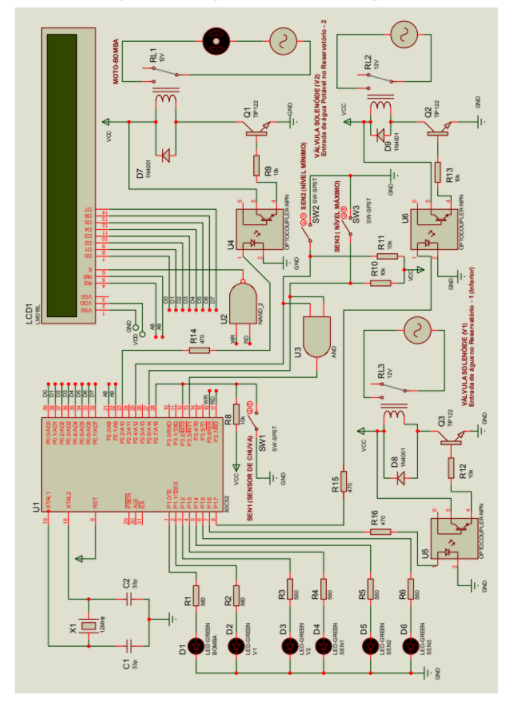
\includegraphics[width=0.5\textwidth, angle=-90]{figuras/trabalhos_relacionados/fig02.png}
	\label{fig:trab_rel_02}
\end{figure}

\begin{figure}[H]
	\centering
	\caption{Microcontrolador \textit{Philips 80C552} acoplado ao kit \textit{CW 552}.}
	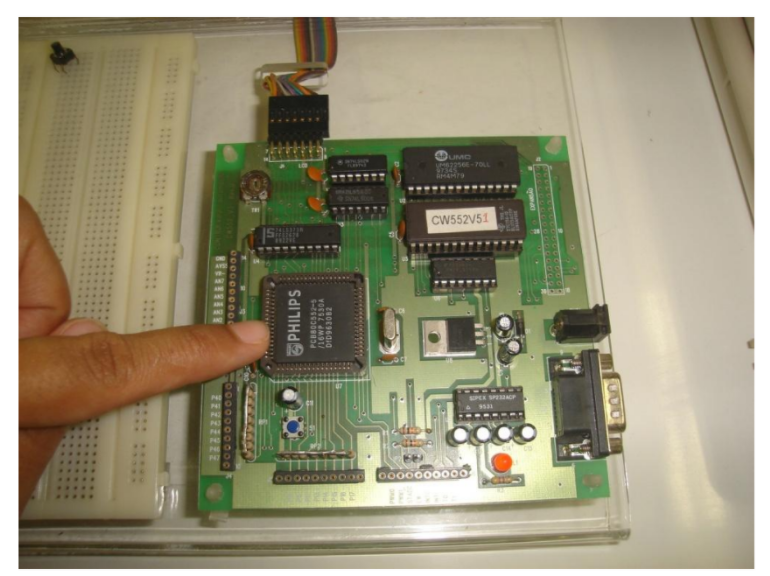
\includegraphics[width=0.5\textwidth]{figuras/trabalhos_relacionados/fig03.png}
	\label{fig:trab_rel_03}
\end{figure}

\newpage

\section{Automação residencial Usando protocolo \textit{MQTT}, \textit{NODE-RED} e \textit{Mosquitto Broker} com \textit{ESP32} e \textit{ESP8266}}

\textbf{Autor:} Victor Ferreira Martins
\vspace{\onelineskip}

Este trabalho de conclusão de curso desenvolvido por Victor Ferreira Martins teve o objetivo de propor uma solução de automação residencial que fosse capaz de integrar três diferentes sistemas em uma casa: monitoramento de temperatura, alarmes de segurança e acionamento de iluminação e tomadas. O objetivo dessa integração foi ajudar a alcançar três dos grandes objetivos da automação residencial: conforto, segurança e economia de energia.
Como caraterísticas importantes destacam-se: a utilização do protocolo\textit{ MQTT} para comunicação através do \textit{Mosquitto Broker}, assim como o uso da ferramenta de programação visual \textit{Node-RED} e dos microcontroladores \textit{ESP32} e \textit{ESP8266}.

Em relação ao trabalho pode-se abstrair os seguintes dados:

\begin{enumerate}
	\item A utilização do protocolo \textit{MQTT}, por meio do \textit{Broker Mosquitto} em conjunto com os microcontroladores da \textit{ESPRESSIF};
	\item A utilização de diversos sensores, validando que a conexão e transferência de dados através do protocolo \textit{MQTT};
	\item Uma abordagem para a organização dos tópicos \textit{MQTT} (\autoref{tab:tabela_topicos}), definindo dispositivos de publicação (\textit{publishers}) e de inscrição (\textit{subscribes});
	\item A utilização do \textit{Node-RED} como agente de interfaceamento do projeto (\autoref{fig:trab_rel_01}).
\end{enumerate}

\begin{figure}[H]
	\centering
	\caption{Visão geral do projeto.}
	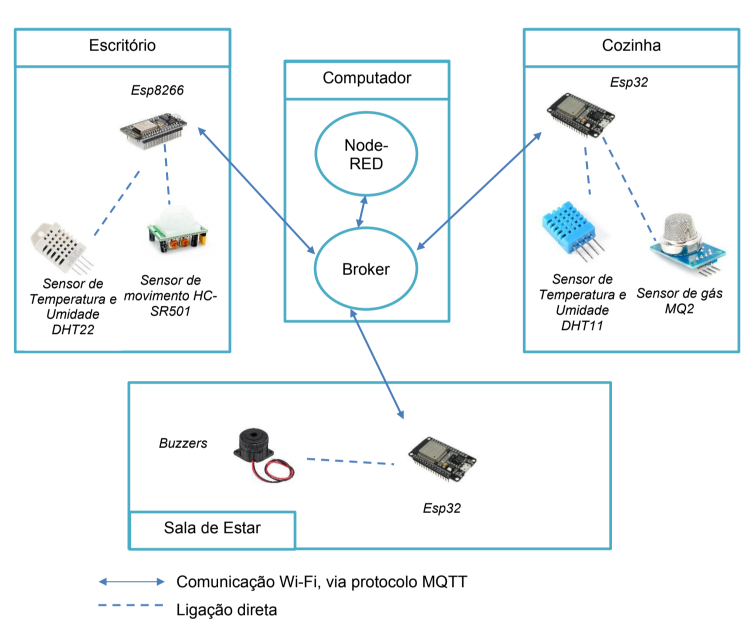
\includegraphics[width=0.8\textwidth]{figuras/trabalhos_relacionados/fig04.png}
	\label{fig:trab_rel_04}
\end{figure}

\begin{figure}[H]
	\centering
	\caption{Visualização da interface desenvolvida no \textit{Node-RED} para receber entradas do usuário e mostrar dados dos sensores.}
	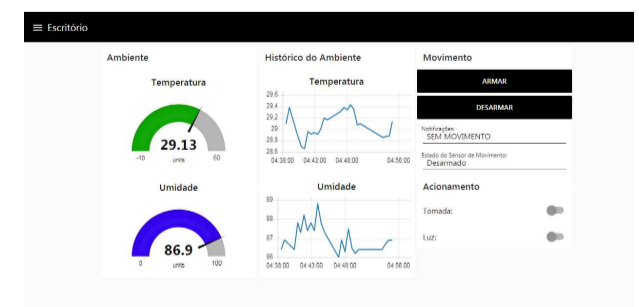
\includegraphics[width=0.8\textwidth]{figuras/trabalhos_relacionados/fig05.png}
	\label{fig:trab_rel_05}
\end{figure}

\begin{table}[H]
	\centering
	\small
	\caption{Organização dos tópicos \textit{MQTT}.}
	\begin{tabular}{c|c|c}
		\hline
		\textbf{Dispositivo} & \textbf{Inscrição} & \textbf{Publicação} \\ \hline
		\multirow{4}{*}{\begin{tabular}[c]{@{}c@{}}ESP8266\\ \\ (Escritório)\end{tabular}} & \multirow{2}{*}{casa/escritório/esp8266/movimento} & casa/escritório/esp8266/temperatura \\ \cline{3-3} 
		&  & casa/escritório/esp8266/umidade \\ \cline{2-3} 
		& casa/escritório/esp8266/tomada & \begin{tabular}[c]{@{}c@{}}casa/escritório/esp8266/movimento/\\ estado\end{tabular} \\ \cline{2-3} 
		& casa/escritório/esp8266/luz & \begin{tabular}[c]{@{}c@{}}casa/escritório/esp8266/movimento/\\ notificação\end{tabular} \\ \hline
		\multirow{4}{*}{\begin{tabular}[c]{@{}c@{}}ESP32\\ (Cozinha)\end{tabular}} & casa/esp32/cozinha/fumaça & casa/cozinha/esp32/temperatura \\ \cline{2-3} 
		& \begin{tabular}[c]{@{}c@{}}casa/cozinha/esp32/\\ tomada\end{tabular} & casa/cozinha/esp32/umidade \\ \cline{2-3} 
		& \multirow{2}{*}{casa/cozinha/esp32/luz} & casa/cozinha/esp32/fumaça/estado \\ \cline{3-3} 
		&  & casa/cozinha/esp32/fumaça/notificação \\ \hline
		\multirow{2}{*}{\begin{tabular}[c]{@{}c@{}}ESP32\\ (Sala de estar)\end{tabular}} & casa/escritório/esp8266/notificação & \multirow{2}{*}{-} \\ \cline{2-2}
		& casa/cozinha/esp32/notificação &  \\ \hline
	\end{tabular}
	\label{tab:tabela_topicos}
\end{table}

\newpage

\section{Desenvolvimento de plataformas embarcadas aplicadas a implementação de \textit{Smart Buildings} com base no \textit{framework SmartLVGrid}}

\textbf{Autor:} Rubens de Andrade Fernandes
\vspace{\onelineskip}

Este trabalho de conclusão de curso desenvolvido por Rubens de Andrade Fernandes pela Universidade do Estado do Amazonas concentrou-se no desenvolvimento de algorítimos para \textit{software} embarcado e dispositivos
de \textit{hardware}, associados a plataformas microcontroladas e microprocessadas, com o objetivo de realizar a convergência \textit{smart building} em sistemas de iluminação e medição de energia elétrica sem recursos de automação, comunicação e controle.

Os pontos relevantes deste trabalho em relação à para implementação deste TCC estão na criação de rotinas de cadastro geradas exclusivamente pelos microcontroladores \textit{ESP32} utilizados (Figura 5.6). 

\begin{figure}[H]
	\centering
	
	\caption{Configuração dos dispositivos}
	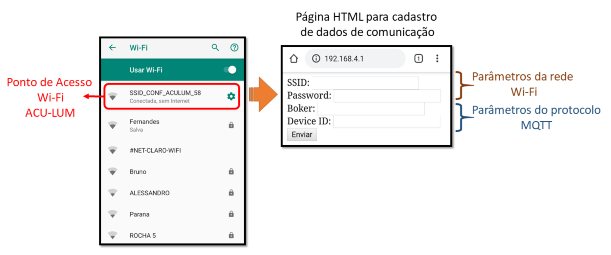
\includegraphics[width=0.8\textwidth]{figuras/trabalhos_relacionados/fig06.png}
	\label{fig:trab06}
\end{figure}

Essa rotina de cadastro faz com que o microcontrolador forneça um ponto de acesso local possibilitando qualquer o acesso de qualquer dispositivo. Ao realizar uma conexão através de um computador ou \textit{smartphone}, por exemplo, o usuário pode informar dados de cadastro como para o dispositivo operar em rede.

O segundo ponto que se pode destacar desse trabalho foi a criação de bibliotecas que auxiliam na operação do microcontrolador como demonstrado na tabela abaixo. 

\begin{table}[H]
	\centering
	\small
	\caption{Bibliotecas implementadas para elaboração do \textit{firmware}}
	\begin{tabular}{cc}
		\hline
		Bibliotecas & Descrição \\ \hline
		DriverAcuLum & \begin{tabular}[c]{@{}c@{}}Utilizada para implementar os métodos referentes\\  as DRFs a serem executadas\end{tabular} \\
		DriverMQTT & \begin{tabular}[c]{@{}c@{}}Utilizada para garantir confiabilidade e \\ segurança no uso do protocolo MQTT\end{tabular} \\
		DriverWIFI & \begin{tabular}[c]{@{}c@{}}Utilizada para garantir uma conexão mais estável, \\ robusta e segura na rede Wi-Fi\end{tabular} \\
		SaveData & \begin{tabular}[c]{@{}c@{}}Utilizada para armazenar os parâmetros do ACU-LUM \\ na EEPROM do ESP32\end{tabular} \\ \hline
	\end{tabular}
	\label{tab:my-table}
\end{table}

Outro ponto importante foi a confecção dos módulos propostos, utilizando técnicas de modelagem 3D para visualização \textit{PCB's} e a realização de soldagem e inserção de componentes.

\begin{figure}[H]
	\centering
	\label{fig:trab_rel_07}
	\caption{Comparação entre o \textit{layout 3D} e o dispositivo físico montado}
	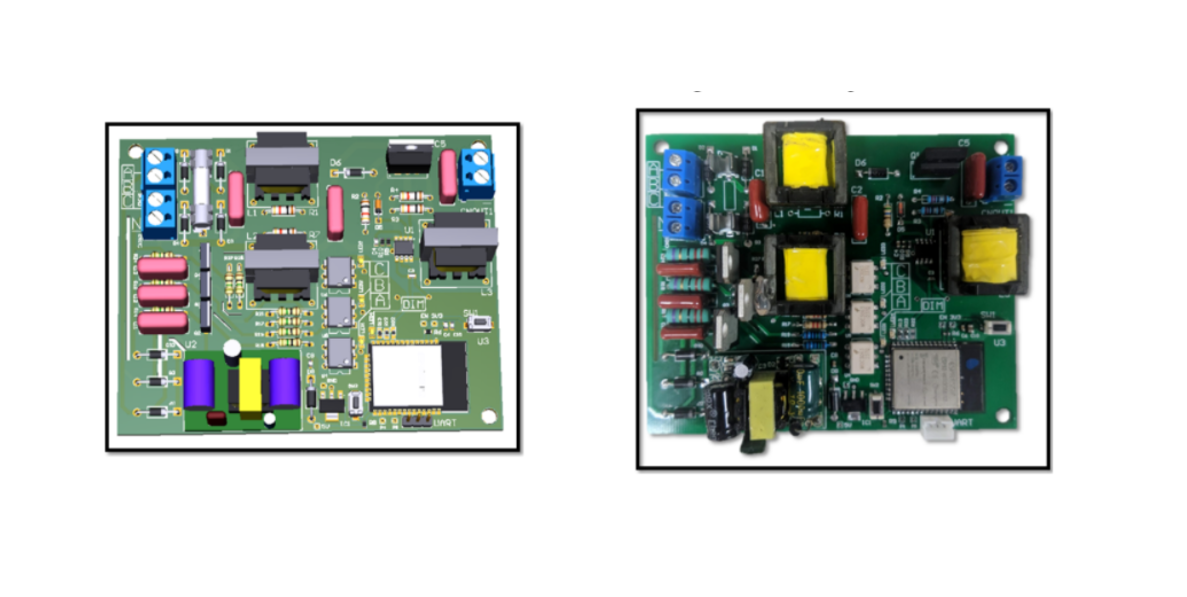
\includegraphics[width=0.5\textwidth]{figuras/trabalhos_relacionados/fig07.png}
	
\end{figure}



\section{Design, Implementation and Practical Evaluation of an IoT Home Automation System for Fog Computing Applications Based on \textit{MQTT} and \textit {ZigBee-WiFi}	Sensor Nodes}

\textbf{Autores:} Iván Froiz-Míguez, Tiago M. Fernández- Camaramés, Paula Fraga-Lamas e Luis Castedo
\vspace{\onelineskip}

Este artigo desenvolvido por membros do departamento de engenharia de computação, da Universidade da Coruña, Espanha, apresentou um estudo de caso e aplicação onde buscou-se unir duas tecnologias dentro das características da \textit{IoT}: \textit{WI-FI} e o protocolo \textit{ZigBee}. O protocolo \textit{ZigBee} é muito utilizado quando se tem a necessidade de uma comunicação à longas distâncias com um baixo consumo energético.

O trabalho apresentou a formulação de uma nova tecnologia: o \textit{ZiWi}, um \textit{HAS - Home Automation System} de computação em nuvem que preenche a lacuna entre dispositivos \textit{ZigBee} e \textit{Wi-Fi}, conectando sensores e atuadores perfeitamente para fazer uso de tais tecnologias em uma residência. O \textit{ZiWi} utiliza o \textit{Wi-Fi} para comunicação com atuadores já que, em geral, há a necessidade de estar continuamente operando e ouvindo comandos assíncronos. Enquanto o \textit{ZigBee} é aplicado para sensores porque é ideal para enviar dados em intervalos periódicos, a fim de economizar energia (já que muitos sistemas dependem de baterias). Além disso, o sistema se concentra no crescente mercado de \textit{IoT} e na utilização de sensores emergentes. Além disso, \textit{ZiWi} faz uso da computação em nuvem, paradigma para fornecer conectividade entre o usuário e os diferentes eletrodomésticos, não apenas
permitindo ao usuário controlá-los, mas também oferecendo a possibilidade dos dispositivos aprenderem com bancos de dados \textit{online}. Isso é alcançado
graças à natureza distribuída do \textit{ZiWi}: o hardware do controlador doméstico é mantido com o mínimo de execuções de tarefas em tempo real, delegando o processamento dos dados e as decisões em tempo não real para servidores em nuvem remotos.

Com a utilização o \textit{Wi-Fi}, o trabalho procurou integrar o protocolo \textit{MQTT} (como a figura de um dispositivo \textit{Broker}, a publicação e inscrição em tópicos) para dispositivos que trabalhavam com o protocolo \textit{ZigBee}. A técnica desenvolvida se tornou muito interessante para aplicações em trabalhos posteriores a esse TCC, como a utilização em ambientes mais isolados.

\begin{figure}[H]
	\centering
	\label{fig:trab_rel_08}
	\caption{Esquema para aplicação do protocolo \textit{ZiWi}}
	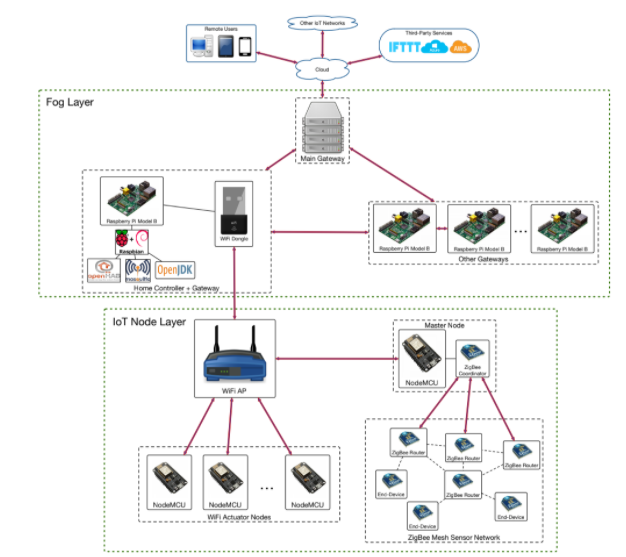
\includegraphics[width=1.0\textwidth]{figuras/trabalhos_relacionados/fig08.png}
	
\end{figure}
 
	% FUNDAMENTAÇÃO TEÓRICA--------------------------------------------------------

\chapter{FUNDAMENTAÇÃO TEÓRICA}
\label{chap:fundamentacao-teorica}

Neste capítulo, serão abordados os aspectos teóricos necessários para o melhor discernimento das definições e componentes a serem utilizados ao longo do projeto. De início, serão abordados os conceitos base como redes \textit{Wireless}, \textit{Internet of Things}, \textit{Smart Things} e o protocolo \textit{MQTT}. Conceitos como a montagem de circuitos eletrônicos, sensoriamento, implementação de sistemas embarcados assim como as tecnologias envolvidas na criação de aplicações \textit{mobile} e \textit{desktop} também serão tratadas neste capítulo. As subseções posteriores, agruparão os conceitos em elementos: de base, de \textit{Hardware},  de \textit{Firmware} e de \textit{Software}.  

\section{Elementos Base}

Esta seção discorre sobre as tecnologias e metodologias que serão utilizadas em todas as vertentes deste trabalho, destacando-se as partes mais relevantes.

\subsection{Redes \textit{Wireless}}

O termo \textit{Wireless} provém do inglês: \textit{wire} (fio, cabo); less (sem); caracteriza qualquer tipo de conexão para transmissão de sem a utilização fios ou cabos \cite{redeswireless}. É importante notar que uma rede sem fio possibilita um conjunto de equipamentos conectados através de sinais de rádio frequência possuindo vantagens cruciais para a aplicação do conceito de Internet das Coisas:

\begin{itemize}
	\item \textbf{Maior produtividade - } disponibiliza acesso à rede em todo o raio de alcance onde o ponto de acesso está instalado, oferecendo liberdade de deslocamento com conexão contínua;
	
	\item \textbf{Flexibilidade de instalação -} podem ser instaladas em locais com temperaturas elevadas, em que os cabos não suportariam, ou em locais que necessitam de acesso temporário;
	
	\item \textbf{Redução de custo - } reduzem os custos de instalação, dispensando o uso de material para cada ponto de conexão;
	
	\item \textbf{Interoperabilidade e segurança - } capaz de comunicar sistemas de forma confiável e com segurança, possuindo chaves de acesso e até mesmo transferindo mensagens criptografadas.   

\end{itemize}

Dentre as diversas características podemos destacar que as redes \textit{wireless} são dividas quanto a \textbf{abrangência de sinal} em:

\begin{itemize}
	\item \textbf{\textit{Wireless Local Area Network} - WLAN - } rede de área local;
	\item \textbf{\textit{Wireless Metropolitan Area Network} - WLAN - } rede de região metropolitana;
	\item \textbf{\textit{Wireless Wide Area Network} - WWAN - } rede de área mundial sem fio;
	\item \textbf{\textit{Wireless Local Loop} - WLL - } acesso fixo sem fio;
	\item \textbf{\textit{Wireless Personal Area Network} - WPAN} - redes pessoais sem fio;
\end{itemize}

Fundado em 1987, o grupo de trabalho \textit{Institute of Electrical and Electronics Engineers} - \textit{IEEE} 802.11\textit{ Wireless LAN}, realizou a padronização das \textit{WLANs}. Desenvolveu-se o padrão DS-SS IEEE 802.11b, chamado de \textit{Wi-Fi} pela \textit{Wireless Ethernet Compatibility Alliance} - WECA o qual é amplamente usado no mercado atual. \cite{internetdascoisassemmisterios}. A partir dessa padronização é possível aplicar as transmissões de dados por diversos protocolos de maneira barata e prática.

A topologia de uma rede IEEE 802.11 (\textit{Wi-Fi})  possui os seguintes elementos-chave:

\begin{itemize}
	\item \textbf{BSS - \textit{Basic Service Set} -} corresponde a uma célula de comunicação \textit{wireless};
	\item \textbf{STA - \textit{Stations} -} são as estações de trabalho que comunicam-se entre si dendo da \textbf{BSS};
	\item \textbf{AP - \textit{Access Point} -} coordena a comunicação entre as \textbf{STA's} dentro da \textbf{BSS}. Na maioria das vezes roteadores realizam tal operação;
	\item \textbf{\textit{Bridge} -} faz a ligação entre diferentes redes, por exemplo, uma rede sem fio para uma rede cabeada convencional;
	\item  \textbf{ESS - \textit{Estended Service Set} -} consiste de várias células \textbf{BSS's} vizinhas que se interceptam e cujos \textbf{AP's} estão conectados a uma mesma rede tradicional. Nestas condições uma \textbf{STA} pode movimentar-se de um \textbf{BSS} para outr, permanecendo conectada à rede. Este processo é denominado \textit{Roaming}.
\end{itemize}

\subsection{A Internet das Coisas}

Existe uma diversidade de ideias em relação ao conceito de Internet das Coisas (\textit{Internet of Things - IoT}), sendo que todos os conceitos, em resumo, fazem alusão à um conjunto de tecnologias e protocolos associados que permitem que objetos se conectem a uma rede de comunicações e onde são identificados e controlados.

Esse termo se tornou possível graças aos avanços tecnológicos e as reduções de custo de todos os dispositivos eletroeletrônicos, os quais possuem a capacidade de comunicação principalmente por meio de protocolos \textit{Wiress} (\autoref{fig:iot_protocols}). Com a aplicação em massa do \textit{IoT} surge a \textit{hiperconectividade}, termo que descreve a possibilidade da aquisição descomunal de informações as quais podem ser utilizadas para melhorar um processo, produto ou serviço.

\begin{figure}[H]
	\centering
	\caption{Protocolos utilizados para aplicacão do \textit{IoT} com base nos conceitos de redes. Relação entre velocidade-força e distância.}
	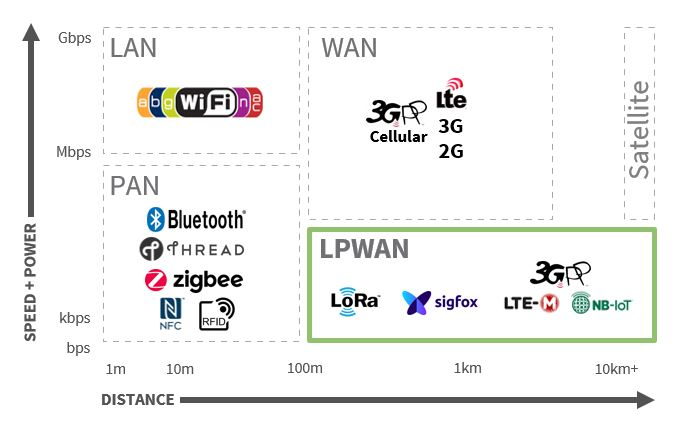
\includegraphics[width=0.8\textwidth]{figuras/iotprotocols.jpg}
	\fonte{iot.do, 2021}
	\label{fig:iot_protocols}
\end{figure}


\subsection{O protocolo MQTT}

O protocolo \textbf{\textit{Message Queuing Telemetry Transport}} - MQTT foi inventado e desenvolvido inicialmente pela \textit{International Business Machines} - IBM no final dos anos 90. Sua aplicação original era vincular sensores em \textit{pipelines} de petróleo a satélites. 

Como seu nome sugere, ele é um protocolo de mensagem com suporte para a comunicação \textbf{assíncrona} entre as partes. Um protocolo de sistema de mensagens assíncrono desacopla o emissor e o receptor da mensagem tanto no espaço quanto no tempo e, portanto, é escalável em ambientes de rede que não são confiáveis. Apesar de seu nome, ele não tem nada a ver com filas de mensagens, na verdade, ele usa um modelo de publicação e assinatura. No final de 2014, ele se tornou oficialmente um padrão aberto OASIS, com suporte nas linguagens de programação populares, usando diversas implementações de \textit{software} livre \cite{IBM}.

O MQTT foi projetado para aplicações que utilizam pouca banda de rede, com requisitos de \textit{hardware} extremamente simples e leve. Ele está na mesma camada OSI que o \textbf{\textit{Hypertext Transfer Protocol}} - HTTP, porém a maior diferença entre eles é o tamanho do \textit{payload}. No HTTP o \textit{payload} \footnote{\textit{\textbf{payload}} - Dado de interesse sem metadados, sem cabeçalho de transmissão ou outras informações acessórias usadas apenas como infraestrutura para transmitir o que importa.} é maior, o que inviabiliza o uso em conexões de baixa qualidade. Além disso o MQTT possui maior segurança, apresenta mais níveis de serviço, é menos complexo e permite uma comunicação de 1 para N se comparado ao HTTP que também é um protocolo utilizado no universo de Internet das Coisas \cite{UFRJ}.

Em uma rede MQTT existem dois agentes principais: o \textit{\textbf{broker}} e os \textit{\textbf{clients}}. O \textit{broker} é um servidor que centraliza as mensagens dos clientes e as encaminha para os clientes interessados. Já o cliente é um dispositivo ou serviço que tenha capacidade de interagir com o \textit{broker} e trocar mensagens. Podemos exemplificar como tipos de clientes (\autoref{fig:mqtt_diagram}) um sensor, um controlador, um atuador ou até mesmo um \textit{software} sendo executado em alguma instância da rede.

\begin{figure}[H]
	\centering
	\caption{Diagrama básico MQTT}
	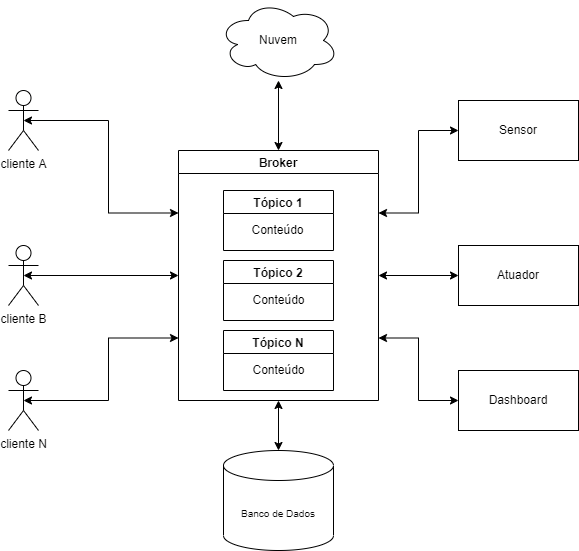
\includegraphics[width=0.8\textwidth]{figuras/mqtt.drawio.png}
	\fonte{própria, 2021}
	\label{fig:mqtt_diagram}
\end{figure}

Como qualquer outro protocolo de comunicação o MQTT possui diversos termos e características associadas, como a segurança, a definição dos \textit{endpoints}\footnote{\textbf{endpoints} - Pontos de extremidade. Terminais de conexão entre uma API e o cliente.}, o endereçamento, tipo de dado trafegado, entre outros. Abaixo estão pontuados os dados cruciais para a aplicação deste trabalho.

\begin{itemize}
	\item \textbf{\textit{broker}}: é o intermediário no processo de comunicação, atuando como um servidor;
	\item \textbf{\textit{client}}: responsável por estabelecer e manter uma conexão com o \textit{broker}, enviar e receber as mensagens;
	\item \textit{\textbf{broker ip}}: identificação única do servidor \textit{\textbf{broker}} conectado em determinada rede;
	\item \textbf{\textit{broker username e broker password}}: credenciais, opcionais, para determinado cliente estabelecer conexão com o servidor; 
	\item  \textit{\textbf{QoS}}: nível de qualidade do serviço desejado, indicando como deve ser a relação entre os elementos comunicantes. \textit{QoS 0}: Não há a confirmação de entrega de uma mensagem e quem a envia não tem obrigação de manter a mensagem armazenada para futuras retransmissões. \textit{QoS 1}: Existe a confirmação de entrega da mensagem. As mensagens enviadas são armazenadas por quem as envia. \textit{QoS 2}: Garante que a mensagem seja entregue exatamente uma vez, com envio de confirmações de recebimento e confirmações de recebimento de confirmações de recebimento. Enquanto uma mensagem não é confirmada, ela é mantida.\cite{fabiobrandao}
	
	\item \textbf{\textit{last good message}}: é a operação à qual o \textit{broker} envia a última menagem válida recebida em um determinado tópico ao ser requisitado por um cliente. Normalmente, se um cliente MQTT assina um tópico em um \textit{broker}, ele não receberá nenhuma das mensagens publicadas nele antes da assinatura. Se um cliente publicar uma mensagem em um tópico com o sinalizador de retenção definido como \textit{True}, o corretor salvará essa mensagem como a “Última Mensagem válida” nesse tópico. Esta mensagem será recebida por qualquer cliente que assine esse tópico \cite{mntolia}. 
	
	\item \textbf{\textit{last will testament (LWT)}}: são mensagens pré-definidas a serem publicadas pelo broker em nome de um determinado cliente, uma vez que esse cliente está \textit{offline} e não pode publicar mais.
	\item \textbf{\textit{keep alive}}: mensagens periódicas enviadas por determinado cliente buscando validar a conexão;
	\item \textbf{tópicos, \textit{publish} e \textit{subscribe}}: O ato de um cliente enviar uma mensagem é chamado \textit{publish}(publicação). E para receber mensagens de determinado um tópico um cliente deve fazer um \textit{subscribe}(inscrição). Os níveis de um tópico são separados por “/” e um cliente pode optar por se inscrever em quantos tópicos forem necessários, utilizando os artifícios da \autoref{tab:simbolos_mqtt}.
	
\end{itemize}

\begin{table}[H]
	\centering
	\resizebox{\textwidth}{!}{%
		\begin{tabular}{c|c|c}
			\hline
			Símbolos & Descrição & Exemplo \\ \hline
			+ & Retorna ou envia qualquer informação naquele nível (Coringa) & \begin{tabular}[c]{@{}c@{}}area/10/sensor/5000/temperatura\\ area/10/sensor/4000/temperatura\\ area/10/sensor/+/temperatura\end{tabular} \\ \hline
			\# & Retorna ou envia qualquer coisa abaixo daquele nível & area/10/\# \\ \hline
			\$ & Tópicos iniciados com \$ são especiais usados internamente pelo broker. & \$SYS/broker/clients/total \\ \hline
		\end{tabular}%
	}
	\caption{Caracteres especiais utilizados para envio e recebimento no protocolo MQTT.}
	\label{tab:simbolos_mqtt}
\end{table}

\section{Elementos de \textit{Hardware}}
\subsection{O microcontrolador ESP8266}

O \textit{ESP8266} (\autoref{fig:esp8266ex}) é um \textit{chip} microcontrolador da fabricante chinesa \textit{Espressif Systems} construído em torno de um processador Tensilica Xtensa LX3, inclui \textit{Wi-Fi on-board}. Originalmente concebido como um adaptador \textit{UART} para \textit{Wi-Fi} (utilizado em \textit{tablets}), permitindo que outros microcontroladores se conectem a uma rede \textit{Wi-Fi} e façam conexões \textit{TCP/IP} simples usando comandos do estilo \textit{Hayes}\footnote{\textbf{comandos \textit{Hayes}:} série de \textit{strings} curtas que podem ser combinadas para produzir comandos de operações como discar, desligar e alterar os parâmetros de conexão.}, o \textit{ESP8266} rapidamente se tornou popular como um microcontrolador autônomo devido ao seu baixo custo de mercado.

\begin{figure}[H]
	\centering
	\caption{\textit{ESP8266EX}.}
	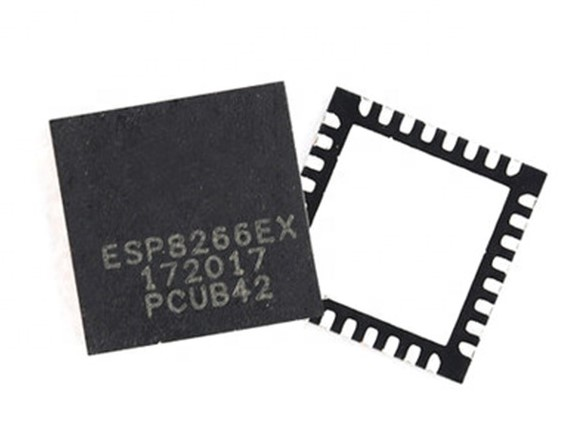
\includegraphics[width=0.3\textwidth]{figuras/esp8266ex.jpg}
	\fonte{DIGIKEY, 2020}
	\label{fig:esp8266ex}
\end{figure} 

Apesar da falta de documentação inicial, uma grande comunidade foi formada em
torno do ESP8266, integrando e dando suporte ao \textit{firmware} para o chip, fazendo-o compatível com a plataforma \textit{Arduino}.
Embora o chip \textit{ESP8266} seja feito pela \textit{Espressif}, existem diversos módulos criados para aplicações distintas.

Os modelos podem se diferenciar pela quantidade de pinos extenados, memória \textit{flash} instalada, modelo de antena, entre outros. Para a realização deste trabalho foram escolhidos os modelos: \textit{ESP-12S} (\autoref{fig:esp12s}) e \textit{ESP-12E} (\autoref{fig:esp12e}) presentes, respectivamentes nas placas de desenvolvimento WEMOS D1 e NodeMCU. Ambos possuem 11 \textit{GPIOs - General Purpose Input Output} sendo ideais para a leitura de uma gama de sensores. A diferença entre ambos está no desenho da antena integrada, sendo a do ESP-12S mais otimizada e, na quantidade de pinos externados, o ESP-12S não extena os pinos voltados para conexão \textit{SPI} e de cartões \textit{SD} \cite{esp8266}. As características gerais e específicas para o densenvolvimento deste trabalho estão descritas no \textbf{anexo A}. 


\begin{figure}[H]
	\centering
	\caption{Vista superior do \textit{ESP-12S}.}
	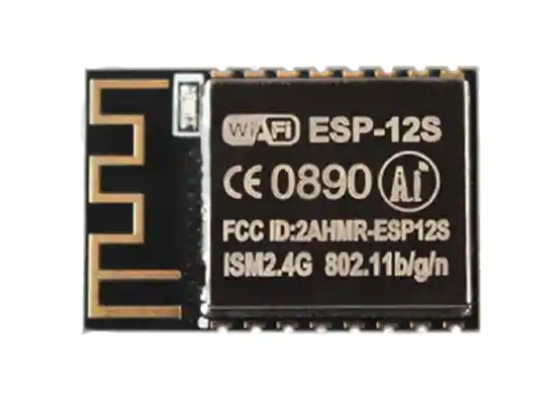
\includegraphics[width=0.3\textwidth]{figuras/ESP-12S.png}
	\fonte{FILIPEFLOP, 2020}
	\label{fig:esp12s}
\end{figure} 

\begin{figure}[H]
	\centering
	\caption{Vista superior do \textit{ESP-12E}.}
	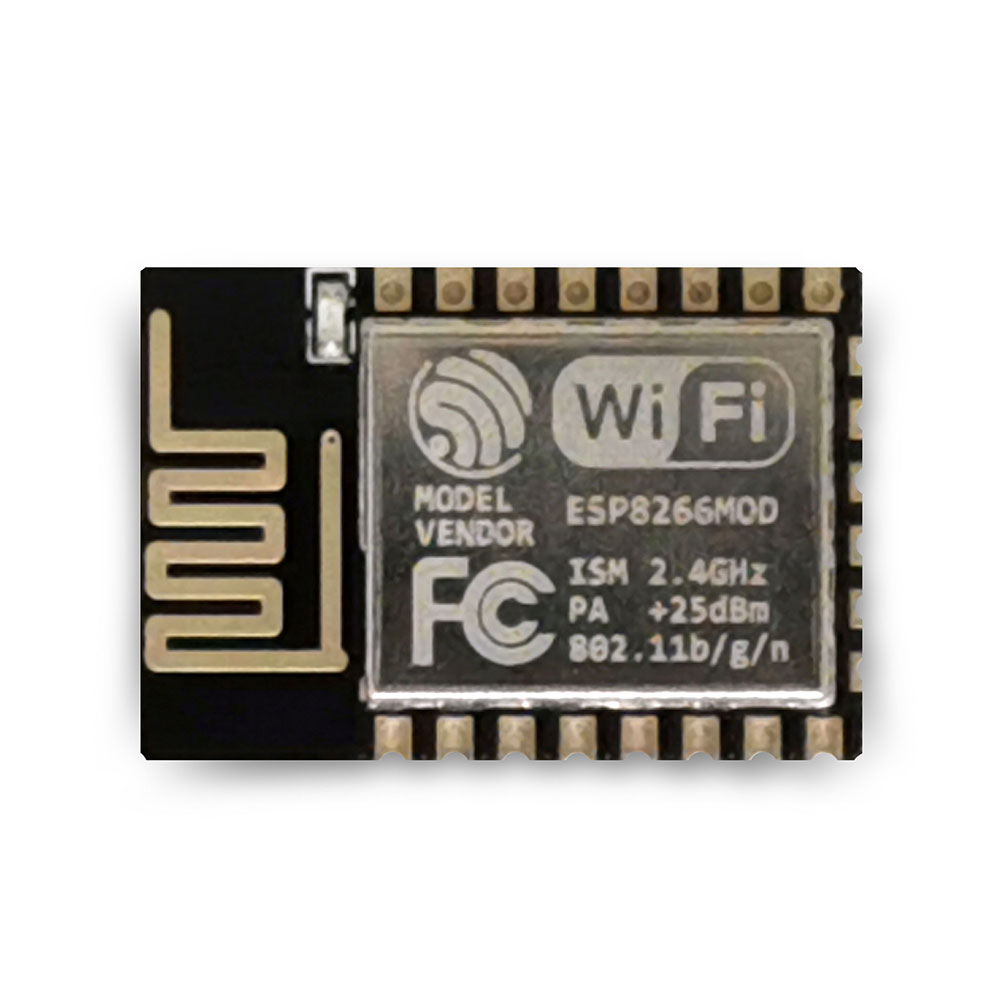
\includegraphics[width=0.3\textwidth]{figuras/ESP-12E.png}
	\fonte{FILIPEFLOP, 2020}
	\label{fig:esp12e}
\end{figure}

\begin{figure}[H]
	\centering
	\caption{Wemos D1 com ESP-12S.}
	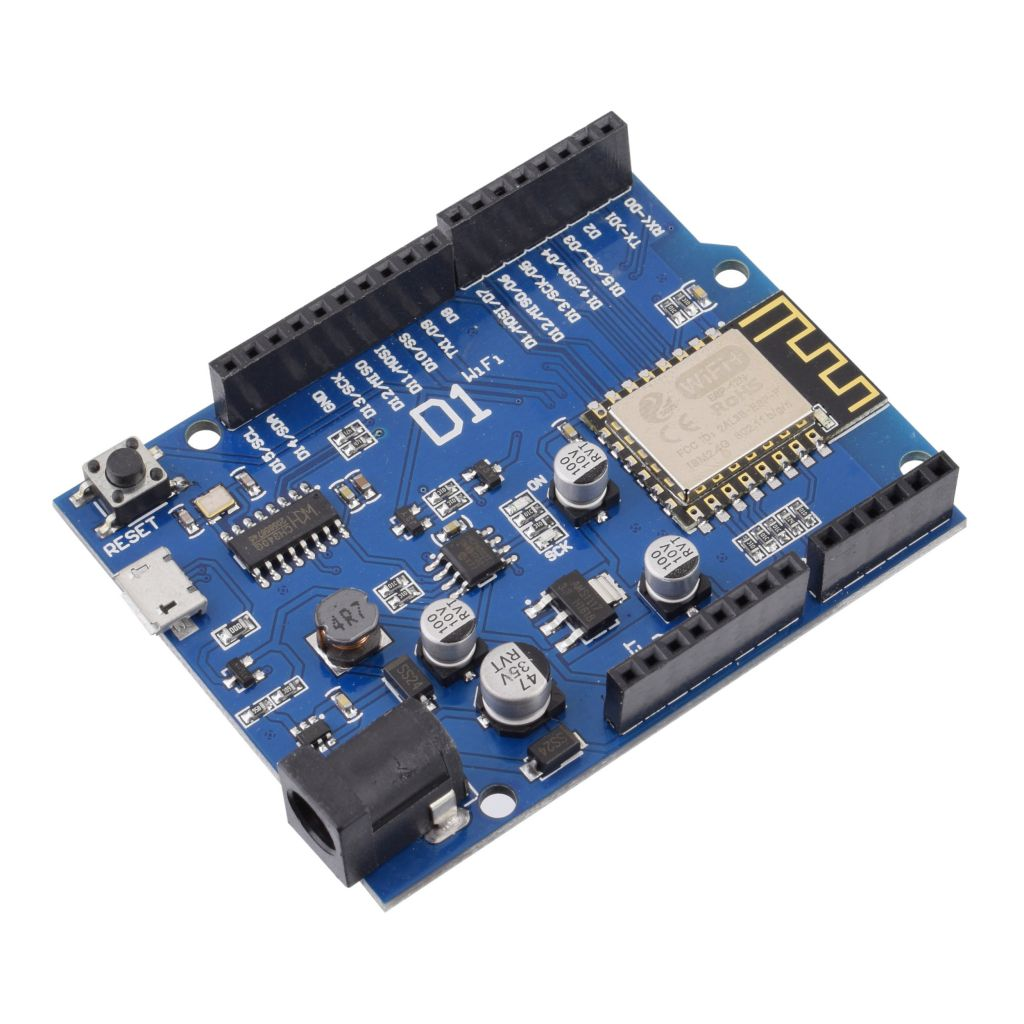
\includegraphics[width=0.3\textwidth]{figuras/ESP-12S-wemos.png}
	\fonte{esp8266.org, 2021}
	\label{fig:esp12s-wemos}
\end{figure}

\begin{figure}[H]
	\centering
	\caption{Nodemcu com ESP-12E.}
	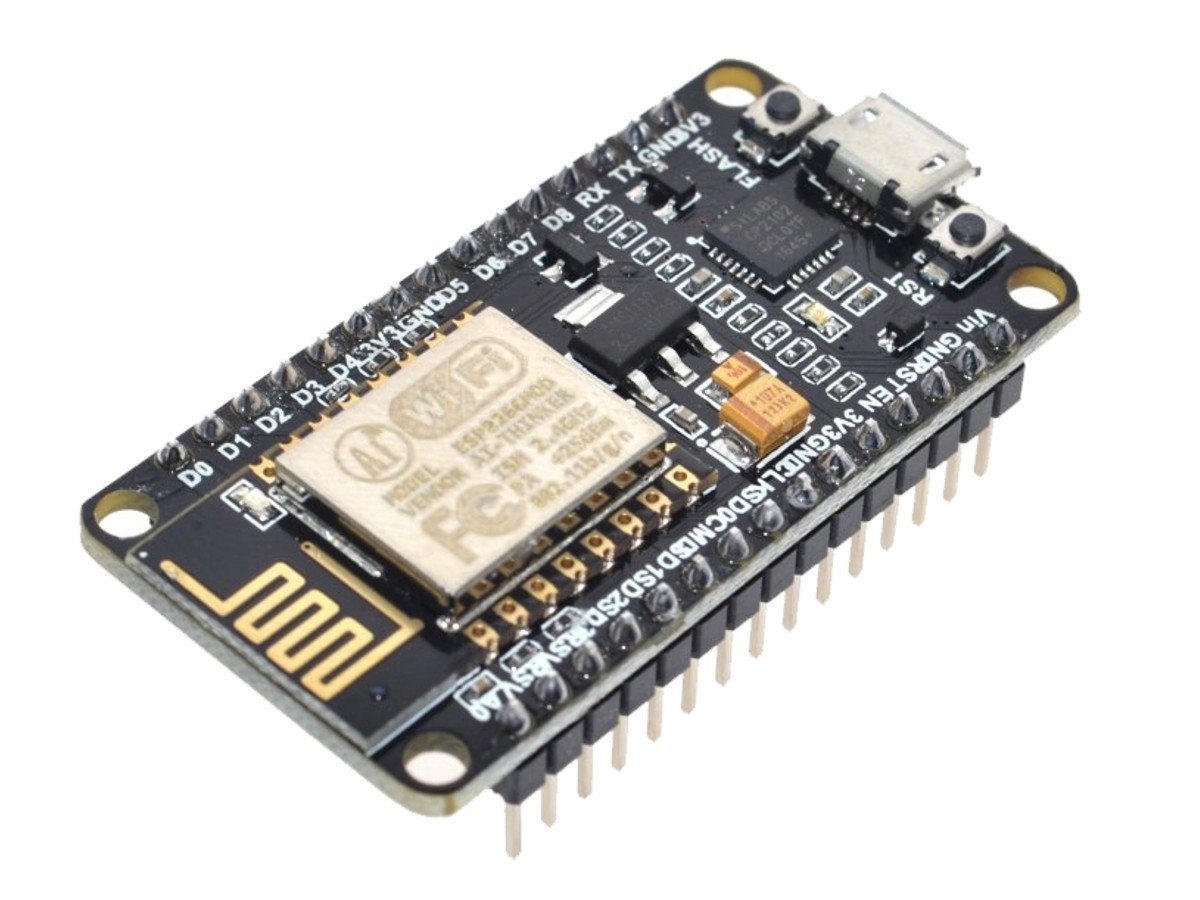
\includegraphics[width=0.3\textwidth]{figuras/ESP-12E-nodemcu.png}
	\fonte{esp8266.org, 2021}
	\label{fig:esp12s-nodemcu}
\end{figure}







\subsection{A Raspberry Pi Zero W}

A \textit{Raspberry Pi Zero W} é basicamente um computador de placa única. Ela possui recursos como \textit{slot} para cartão \textit{microSD}, conectores \textit{HDMI} e de câmera, conectividade \textit{Wi-Fi} e \textit{Bluetooth 4.0}, um conector macho de entrada-saída (\textit{GPIO}) de 40 pinos e mini conector de alimentação \textit{+ 5VDC}. O microcontrolador baseado no processador \textit{BCM2835 ARMv7 system-on-chip (SoC)} alimenta o Pi Zero W.

Essa versão de \textit{hardware} da \textit{Raspberry Pi Foundation} é muito compacta, ficando no meio termo entre as fazes de prototipação e aplicação. Com o microprocessador \textit{ARM BCM2835} de \textit{1GHz}, memória \textit{RAM} de \textit{512MB} e um sistema operacional enxuto instalado, a \textit{Raspberry Pi Zero W} é ideal para rodar aplicações como um \textit{Broker MQTT}. Informações adicionais sobre esse dispositivo estão disponíveis no \textbf{Anexo B}.

\begin{figure}[H]
	\centering
	\caption{Vista superior da \textit{Raspberry Pi Zero W}}
	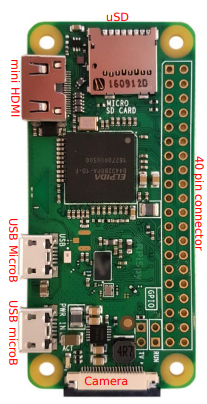
\includegraphics[width=0.3\textwidth, angle = 90]{figuras/rasp_zerow.png}
	\fonte{SPARKFUN, 2020}
	\label{fig:rasppizerow}
\end{figure} 

\subsection{As fontes de alimentação DC}

Para alimentação elétrica de todos os dispositivos eletrônicos envolvidos no processo de automação da cisterna, foram utilizadas dois tipos de fontes chaveadas: de \textit{12V/20A} para o módulo \textbf{CCM} e \textit{12V/10A} para o módulo \textbf{TCM}, representadas pela \autoref{fig:fontechaveada}. Essas fontes são ideais por possuir características robustas, como proteção eletromecânica e potência necessária para ativação de motores e válvulas solenoides. Há também a disponibilização de vários conectores na saída, os quais podem ser interligados para pontos específicos de alimentação.

\begin{figure}[H]
	\centering
	\caption{Vista superior da fonte}
	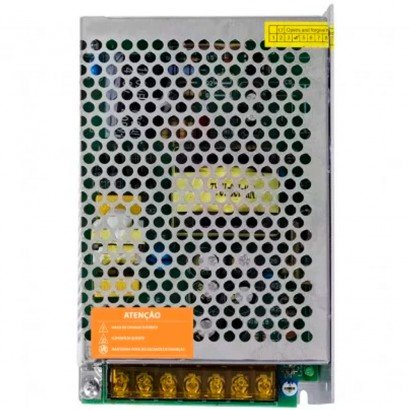
\includegraphics[width=0.4\textwidth]{figuras/fonte_chaveada.jpg}
	\fonte{AMAZON, 2020}
	\label{fig:fontechaveada}
\end{figure} 

\subsection{A motobomba ou bomba d'água}

A bomba d'água selecionada, \autoref{fig:bomba} , trabalha com fontes de alimentação de correntes contínuas (\textit{DC}) o que permite um maior controle do funcionamento através de sistemas \textit{microprocessados}. Essa bomba opera a \textit{12V}, com potência máxima de \textit{80W}. Ela possui a capacidade de exercer uma vazão de \textit{5,5L/min} com ganho de elevação de no máximo 40\textit{m}.

\begin{figure}[H]
	\centering
	\caption{Bomba d'água \textit{DC}}
	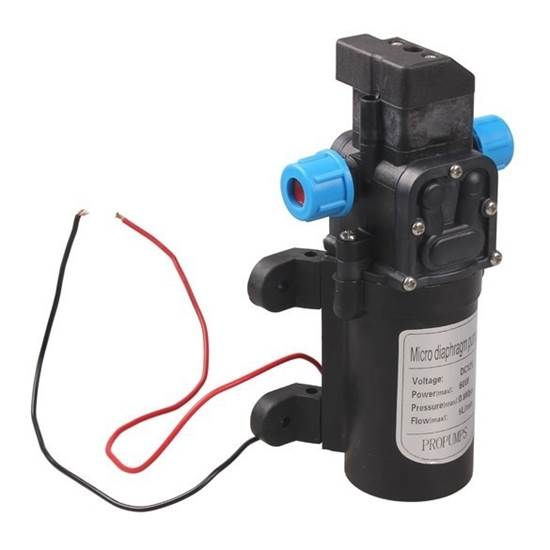
\includegraphics[width=0.3\textwidth]{figuras/bomba.jpeg}
	\fonte{ENERGIA TOTAL, 2020}
	\label{fig:bomba}
\end{figure}

\subsection{O sensor ultrassônico}
\label{ssec:sensor_ultra}

Um sensor ultrassônico é um instrumento que mede a distância até um objeto usando ondas sonoras de frequência acima do alcance da audição humana (ultrassônicas). Ele usa um transdutor para enviar e receber pulsos ultrassônicos os quais são utilizados para medição de distância através de lapsos temporais (\autoref{fig:operacao_ultrassonico}). A equação de distância associada é dada por:

\begin{equation}
d = \frac{\Delta t \cdot v}{2}
\end{equation}
\\
\begin{itemize}
	
	\item $d$ é a distância;
	\item $\Delta t$ é a diferença entre o tempo de emissão e chegada da onda;
	\item  $v$ é a velocidade do som (tomada como $340m/s$). \\
\end{itemize}





\begin{figure}[H]
	\centering
	\caption{Representação do funcionamento de um sensor ultrassônico}
	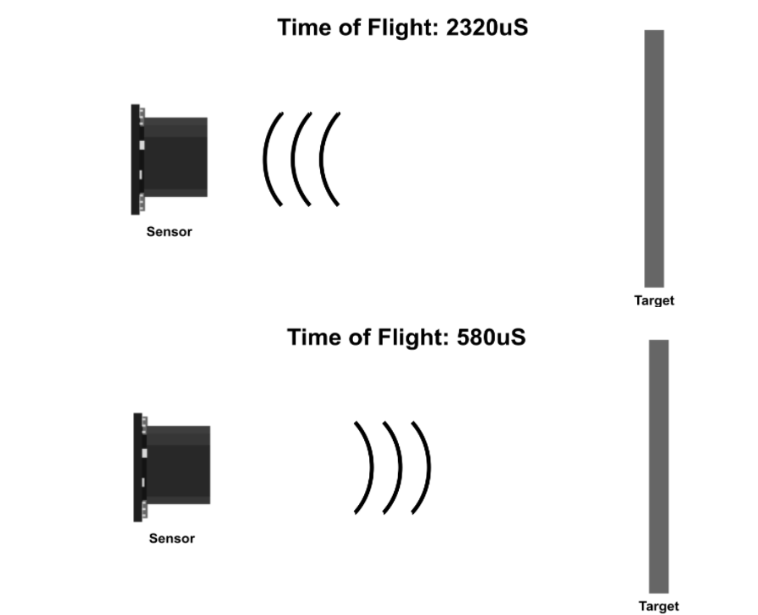
\includegraphics[width=0.6\textwidth]{figuras/ultrassonico_operacao.png}
	\fonte{Maxbotix, 2021}
	\label{fig:operacao_ultrassonico}
\end{figure}

Para medição de nível selecionou-se o módulo ultrassônico \textit{JSN-SR04T}. Esse módulo oferce uma região de medição de distância entre $20 cm$ a $600 cm$, com precisão na faixa de $2 mm$.

Esse módulo de apenas quatro pinos: \textit{5V} (VCC), \textit{Trig (RX)}, \textit{Echo (TX)} e \textit{GND}, inclui um transceptor integrado além do seu circuito de controle o qual possui três modos de operação sendo selecionados pelo valor do resistor (R27) soldado a placa:


\begin{itemize}
	\item \textbf{Modo de operação 1 (R27 não soldado)}: neste modo, o microcontrolador na placa não é utilizado. As operações de leitura ficam por responsabilidade externa. 
	
	\item \textbf{Modo de operação 2 (R27 $= 47k\Omega$)}: neste modo, o microcontrolador da placa entra em modo de leitura constante e envia dados a cada $100ms$. Os dados são enviados via o pino TX respeitando o protocolo: 0XFF + HIGH DATA + LOW DATA + SUM 1.
	
	\item \textbf{Modo de operação 3 (R27 $= 120k\Omega$)}: neste modo, o microcontrolador entra em modo de baixo consumo e só envia os dados de leituras ao ser acionado pelo pino RX. Se a mensagem de acionamento for 0X55, a leitura de distância é enviada pelo TX da mesma forma do modo anterior. \\
\end{itemize}

Sobre o protocolo utilizado, cada parte da mensagem tem a seguinte definição:

\begin{itemize}
	\item 0xFF: indica a chegada de uma mensagem;
	\item HIGH DATA: 8 bits mais significativos da leitura;
	\item LOW DATA: 8 bits menos significativos da leitura;
	\item SUM 1: O resultado da soma de todos os caracteres (0XFF + HIGH DATA + LOW DATA) para que a mensagem seja validada.
\end{itemize}



\begin{figure}[H]
	\centering
	\caption{Sensor ultrassônico JSN-SR04T.}
	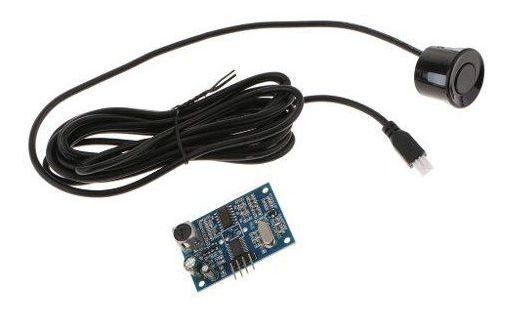
\includegraphics[width=0.5\textwidth]{figuras/sensor_ultra.jpg}
	\fonte{USINAINFO, 2020}
	\label{fig:sensor_ultra}
\end{figure}

O transceptor, resistente à água e poeira, é conectado ao módulo por meio de um cabo com \textit{2,5 metros} de comprimento. 


\subsection{A válvula solenoide}

Uma válvula solenoide (\autoref{fig:valvula_solenoide}) é um tipo de válvula que pode ser acionada ou desacionada eletronicamente. Seu componente principal é uma bobina elétrica com um núcleo ferromagnético móvel no centro chamado de êmbolo.

Dependendo da aplicação, uma válvula pode ser classifica em \textbf{Normalmente Aberta - NA} ou\textbf{ Normalmente Fechada - NF}. Para uma \textbf{NF}, em sua posição de repouso, o êmbolo tampa um pequeno orifício por onde é capaz de circular um fluído. Quando uma corrente elétrica circula na bobina, cria um campo magnético o qual exerce força sobre o êmbolo. Ele é deslocado em direção ao centro da bobina, abrindo o orifício e possibilitando a passagem do fluído. A operação para uma válvula \textbf{NA} é justamente o oposto, o êmbolo fica no centro e é deslocado com a formação do campo magnético. Outra classificação é quanto ao número de vias e as formas de controle. Para este trabalho nos atentaremos para válvulas de duas vias com retorno por mola, representadas na figura abaixo.

\begin{figure}[H]
	\centering
	\caption{Representação de válvulas: \textit{(a)} Normalmente Fechada  e \textit{(b)} Normalmente Aberta. Ambas de duas vias.}
	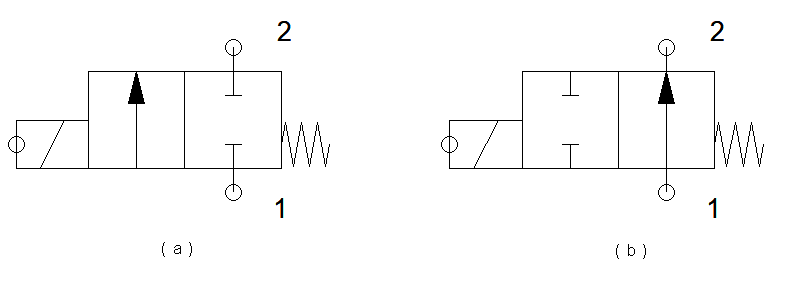
\includegraphics[width=0.7\textwidth]{figuras/valvulas.png}
	\fonte{Própria, 2021}
	\label{fig:valvulas}
\end{figure}

\begin{figure}[H]
	\centering
	\caption{Representação interna de uma válvula solenoide com seus principais componentes}
	\includegraphics[width=0.4\textwidth]{figuras/válvula_solenoide.png}
	\fonte{Citisystems, 2021}
	\label{fig:valvula_solenoide}
\end{figure}

Alguns exemplos do uso de válvulas solenoides incluem sistemas de aquecimento, tecnologia de ar comprimido, automação industrial, piscinas, sistemas de aspersão, máquinas de lavar roupa, equipamentos odontológicos, sistemas de lavagem de carros e sistemas de irrigação \cite{Citisystems}.

O modelo de válvula solenoide utilizada foi da marca Nascimetal (\autoref{fig:solenoide}) a qual possui características como:  \textit{1/2"} x \textit{1/2"}, tensão de operação em torno de \textit{12V} \textit{DC}, consumo médio, quando ativada, de \textit{500mA}, pressão de operação à $8,0 kgf/cm^2$ com vazão máxima de $40L/min$ e vida útil de 50 mil operações. Garantiu o controle do fluxo de água de acordo com os dados elétricos enviados pelo microcontrolador.

\begin{figure}[H]
	\centering
	\caption{Válvula solenoide}
	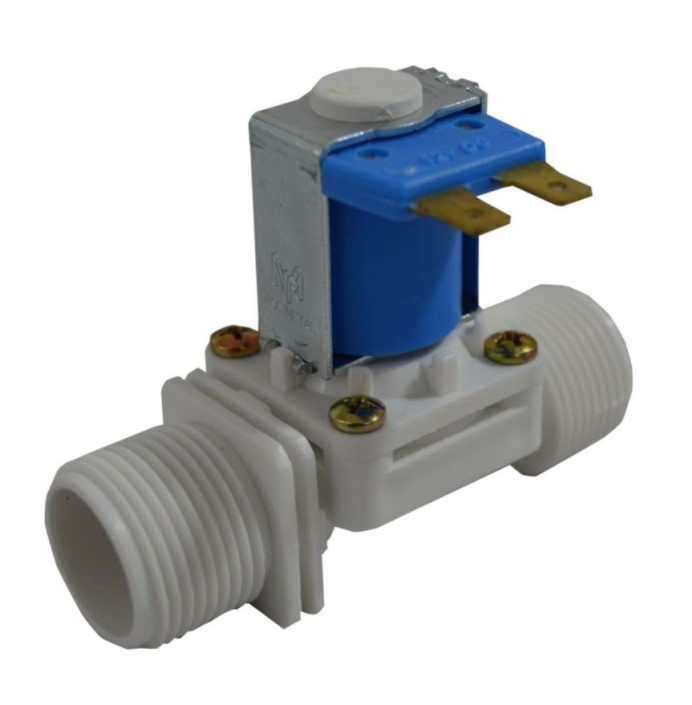
\includegraphics[width=0.3\textwidth]{figuras/solenoide.jpg}
	\fonte{Nascimetal, 2021}
	\label{fig:solenoide}
\end{figure}

\subsection{A chave de nível tipo boia}

Para questões de segurança a chave de nível \textit{RF-0H21D} foi utilizada para fomentar a redundância do sistema, caso aconteçam falhas na medição do sensor citado na seção \ref{ssec:sensor_ultra}. Essa chave indicará para o microcontrolador, por meio de contato elétrico, o momento exato para desativação da bomba d'água, evitando possíveis vazamentos no sistema acolado à caixa d'água (\textbf{TCM}). 

\begin{figure}[H]
	\centering
	\caption{Chave de nível \textit{RF-0H21D}}
	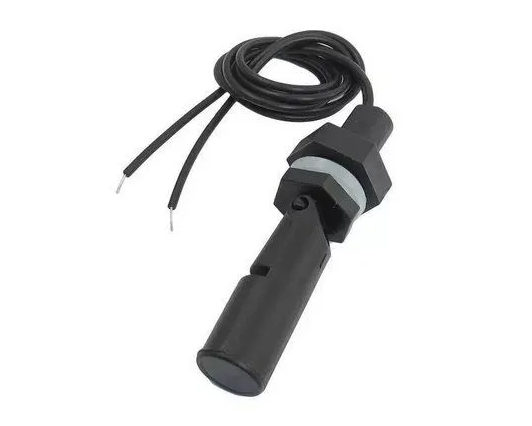
\includegraphics[width=0.5\textwidth]{figuras/chave_boia.png}
	\fonte{SMART KITS, 2020}
	\label{fig:chaveboia}
\end{figure}


\subsection{O sensor de corrente}

O sensor de corrente ACS712 selecionado é acessível e oferece precisão em soluções para detecção de corrente AC ou DC na indústria,
comercial e sistemas de comunicação. O dispositivo permite fácil implementação: aplicações típicas incluem controle de motor, detecção de carga e gerenciamento, fontes de alimentação comutadas e sobrecorrente proteção contra falhas \cite{ACS712}.


\begin{figure}[H]
	\centering
	\caption{Representação gráfica do sensor \textit{ACS712}}
	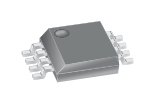
\includegraphics[width=0.3\textwidth]{figuras/ACS712.png}
	\fonte{ALEGRO, 2020}
	\label{fig:acs712}
\end{figure} 


O dispositivo consiste em um operador \textit{Hall} linear preciso, a corrente aplicada flui através do material de cobre gerando um campo magnético que é detectado pelo \textit{Hall} integrado e convertido em um proporcional de tensão. A precisão do dispositivo é otimizada por meio do fechamento proximidade do sinal magnético ao transdutor \textit{Hall}. A resistência interna do material condutor atinge uma média de \textit{1,2m}$\Omega$, proporcionando baixa potência. De acordo \textit{datasheet} do componente, pode-se observar a simples aplicação típica representada na figura abaixo.
 
\begin{figure}[H]
	\centering
	\caption{Aplicação típica do\textit{ACS712}}
	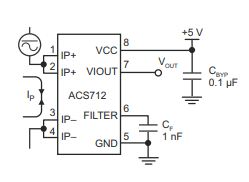
\includegraphics[width=0.4\textwidth]{figuras/ACS712_typical.png}
	\fonte{ALEGRO, 2020}
	\label{fig:acs712_typical}
\end{figure} 

\subsubsection{O sensor \textit{Hall}}

O efeito \textit{Hall} é um fenômeno que pode ser observado quando um dispositivo condutor ou semicondutor se aproxima um campo magnético perpendicular. Nessa situação uma diferença de potencial pode ser medida através dos terminais de tal dispositivo. Essa queda de tensão está relacionada com a intensidade da corrente que gerou o campo magnético \cite{ElectronicsTutorials}. A equação mostra essa relação: 

\begin{equation}
V_H = R_H\left ( \frac{I\cdot B}{t} \right)
\end{equation}

\begin{itemize}
	
	\item $V_H$ é a tensão em Volts;
	\item $R_H$ é o coeficiente do efeito \textit{Hall};
	\item  $I$ é o fluxo de corrente em Amperes;
	\item $t$ é espessura do sensor em milímetros;
	\item $B$ é a densidade do fluxo magnético em teslas; \ \\
\end{itemize}

\begin{figure}[H]
	\centering
	\caption{Comportamento da tensão de saída em relacão ao fluxo magnético de um sensor \textit{Hall}.}
	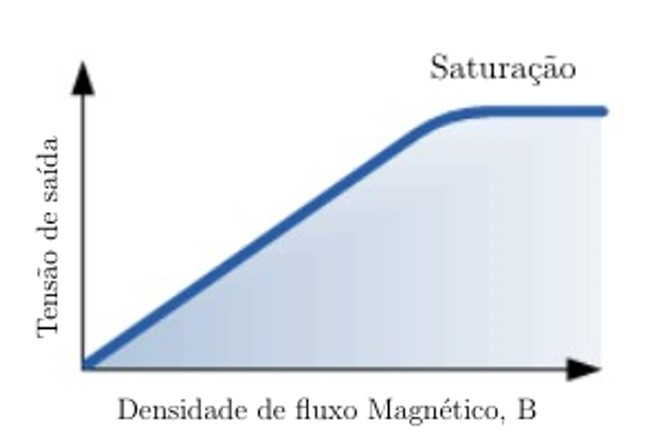
\includegraphics[width=0.4\textwidth]{figuras/grafico_hall.jpg}
	\fonte{Eletronics Tutorials, 2021}
	\label{fig:efeito_hall}
\end{figure} 

Em relação ao sensoriamento, os dispositivos \textit{Hall} podem ser digitais ou analógicos. Os sensores analógicos fornecem uma saída de tensão contínua que de acordo com a intensidade do campo magnético e em alguns casos, como o ACS712, podem apresentar uma variação de saída linear (\autoref{fig:efeito_hall}). Conforme a intensidade do campo magnético aumenta, o sinal de saída do amplificador também aumentará até que comece a saturar pelos limites impostos a ele pela fonte de alimentação do circuito integrado. Essa saída linear pode ser conectada a um pino de leitura analógica de um microcontrolador ou microprocessador.

\subsection{KiCad}

O KiCad é um \textit{Software} de código aberto para projetar circuitos eletrônicos. Essa ferramenta EDA - \textit{Electronic Design Automation} lida com captura esquemática e layout de placas de circuito impresso (PCB - \textit{Printed Circuit Board}) gerando arquivos \textit{Gerber} (padrão universal de arquivo composto de uma combinação de comandos gráficos utilizados por equipamentos tipo \textit{fotoploter} para a formação das imagens da placa de circuito impresso).

O \textit{software} roda em ambientes \textit{Windows}, \textit{Linux} e \textit{OS X} estando licenciado pela GNU GPL v3. Por meio de sua vasta biblioteca é possível construir esquemáticos de maneira prática. O KiCad também possui recursos de criação e adição de componentes, além de simulação via linguagem SPICE (ainda em beta) \cite{Kicad}. 

\begin{figure}[H]
	\centering
	\caption{Exemplo de\textit{PCB Design} utilizando \textit{Kicad}}
	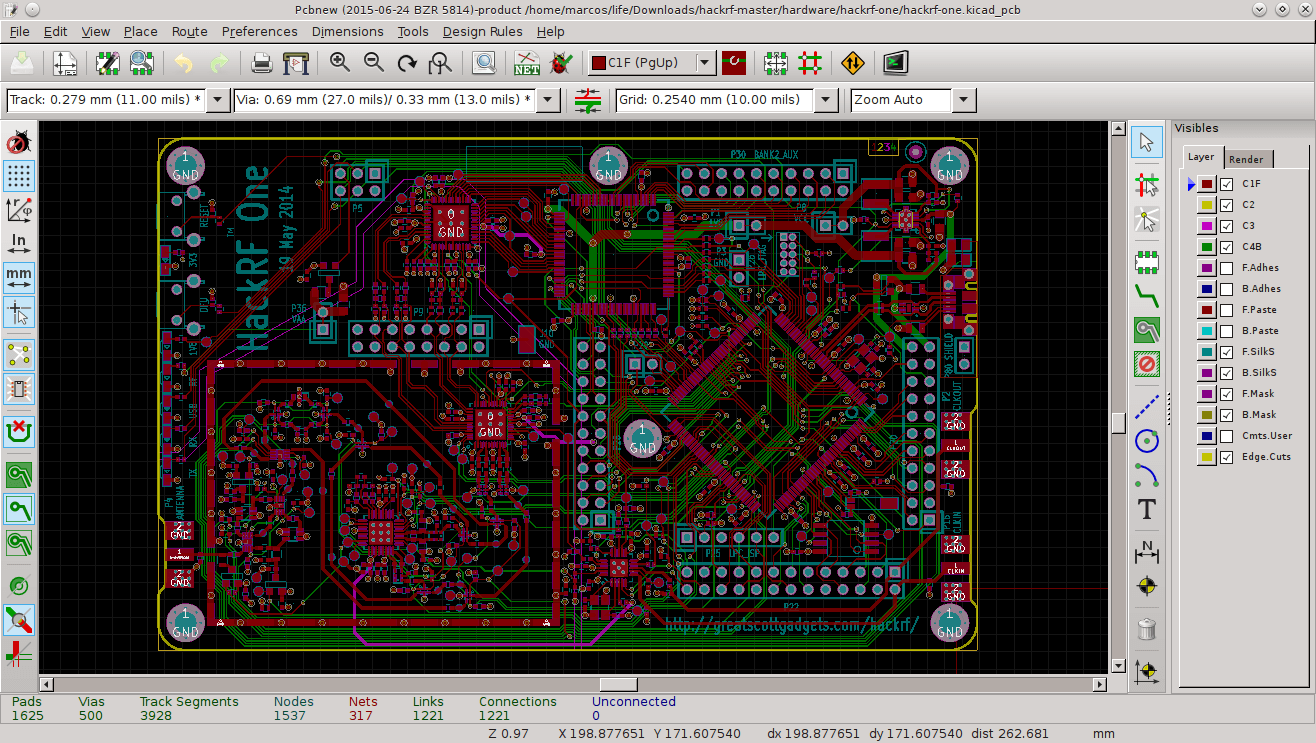
\includegraphics[width=0.6\textwidth]{figuras/kicad_pcbnew.png}
	\fonte{kicad.org, 2021}
	\label{fig:kicad_pcbnew}
\end{figure} 


%\subsection{Autocad Inventor}

\section{Elementos de \textit{Firmware}}

\subsection{O Ambiente de Desenvolvimento \textit{PlatformIO}}


O \textit{PlatformIO} é uma ferramenta profissional de plataforma cruzada, ou seja, disponível em diversas plataformas de desenvolvimento, e de estrutura múltipla voltada para desenvolvedores de \textit{software} embarcado.

A ferramenta (\autoref{fig:platformio}) fornece um ambiente de desenvolvimento integrado moderno, oferecendo suporte a diversos \textit{kits} de desenvolvimento de \textit{software} (\textit{SDKs}) ou \textit{frameworks} e inclui depuração sofisticada (\textit{Debug Mode}), testes de unidade (\textit{Unit Test}), análise automatizada de código (\textit{Static Code Analysis}) e gerenciamento remoto (\textit{Remote Development}). É arquitetado para maximizar a flexibilidade e escolha dos desenvolvedores, que podem usar editores gráficos e/ou de linha de comando (\textit{PlatformIO Core}(\textit{CLI})).

Com esta interface, será possível a programação do microcontrolador \textit{ESP8266} através da linguagem \textit{C++} em conjunto com todas as bibliotecas disponibilizadas pela plataforma Arduino. Todas as funcionalidades, como rotinas de conexão \textit{HTTP} e/ou \textit{MQTT} através do \textit{Wi-Fi}, Interrupção, \textit{Timers} e Modos de Energia são completamente acessíveis. 

\begin{figure}[H]
	\centering
	\caption{Extensão do \textit{PlatformIO} rodando no \textit{Visual Studio Code}}
	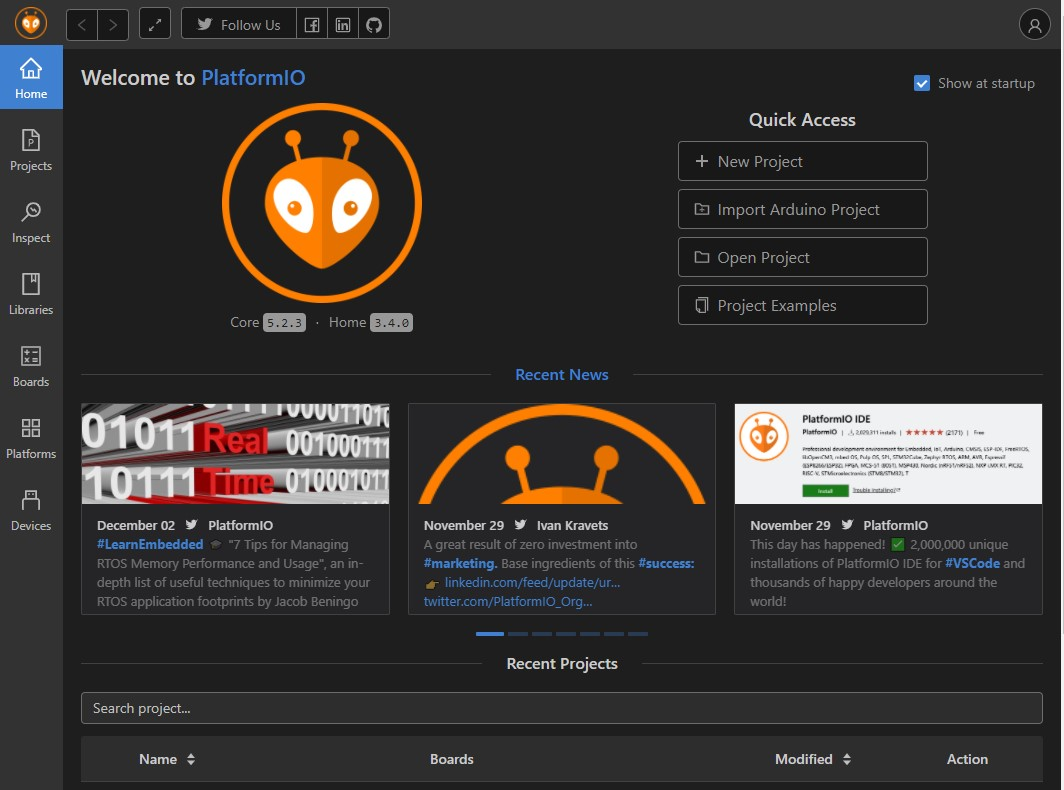
\includegraphics[width=0.7\textwidth]{figuras/platformio.jpg}
	\fonte{Própria, 2021}
	\label{fig:platformio}
	
\end{figure}


\subsection{\textit{Linux} embarcado e a distribuição \textit{DietPi}}

\textit{Linux} é um sistema operacional de código aberto amplamente utilizado em vários sistemas, possuindo compatibilidade com diversos tipos de microprocessadores, sejam eles de arquitetura \textit{Reduced Instruction Set Computer} - RISC ou \textit{Complex Instruction Set Computer} - CISC. Em todos os casos executa rotinas por baixo de todos os outros \textit{softwares}, gerenciando todas as ações em conjunto com \textit{hardware}.

O termo “\textit{Linux}” tecnicamente se refere apenas ao \textit{kernel} do \textit{Linux}. A maioria das pessoas se refere a todo o sistema operacional como \textit{"Linux"} porque, para a maioria dos usuários, um sistema operacional inclui um pacote de programas, ferramentas e serviços (como desktop, relógio, menu de aplicativo e assim por diante). Algumas pessoas, particularmente membros da \textit{Free Software Foundation} , referem-se a esta coleção como \textit{GNU / Linux} , porque muitas ferramentas vitais incluídas são componentes \textit{GNU}. No entanto, nem todas as distribuições do \textit{Linux} usam componentes \textit{GNU} como parte do sistema operacional: o \textit{Android} , por exemplo, usa um \textit{kernel Linux}, mas depende muito pouco das ferramentas \textit{GNU} \cite{opensource}.

O mesmo \textit{Linux} que roda em um supercomputador pode rodar também em uma simples placa eletrônica. O que torna isso possível é que o \textit{Linux} suporta uma grande variedade de arquiteturas e processadores \cite{SoftwareLivre}. Baseado na distribuição em Debian, conhecida por sua alta confiabilidade, a distribuição \textbf{DietPi}, utilizada neste trabalho, é extremamente leve, sendo altamente otimizada para o uso mínimo de recursos de CPU e RAM, garantindo que a \textit{Central Process Unit} - CPU sempre opere em seu potencial máximo. Essa distribuição é suportada por diversos microprocessadores, incluindo o Broadcom BCM2835, presente na Raspberry PI Zero W.

\begin{figure}[H]
	\centering
	\caption{Catálogo com algumas de placas que suportam a distribuição DietPi.}
	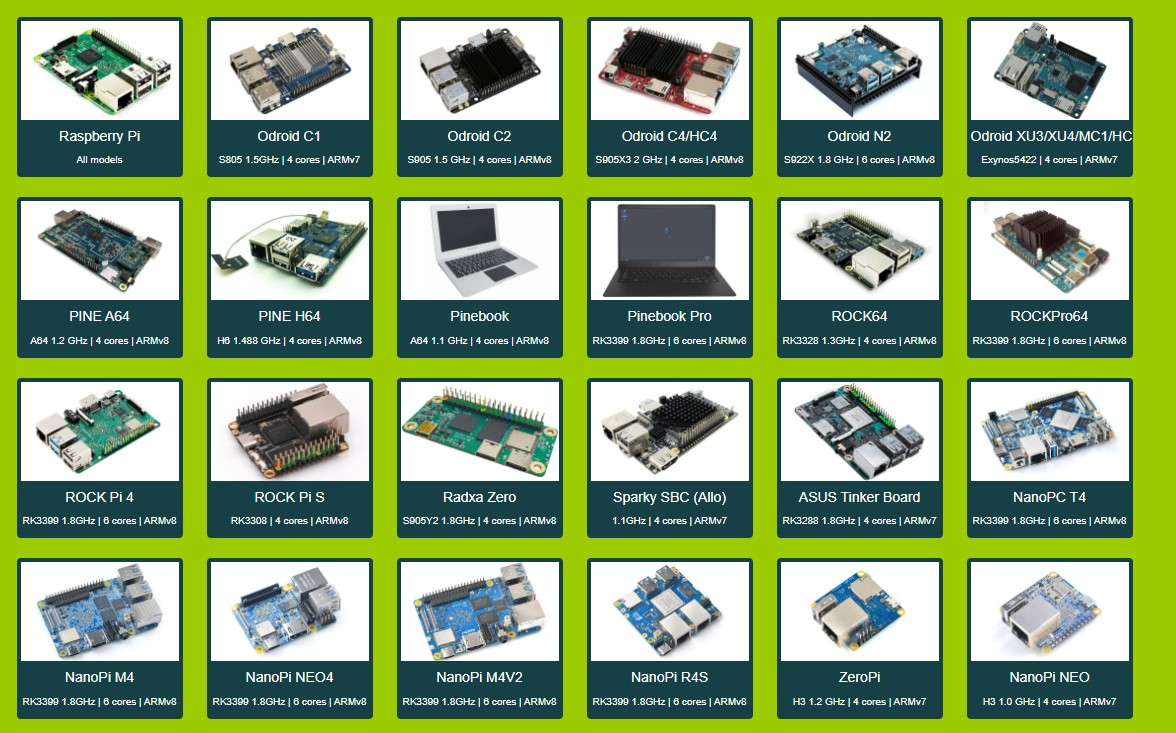
\includegraphics[width=0.7\textwidth]{figuras/dietpi.jpg}
	\fonte{dietpi.com, 2021}
	\label{fig:dietpi}
\end{figure} 


\section{Elementos de \textit{Software}}

\subsection{Figma}

Figma é um editor gráfico de prototipagem para projetos de \textit{design} baseado principalmente no navegador web, com ferramentas \textit{offline} adicionais para aplicações \textit{desktop}, \textit{GNU/Linux}, \textit{macOS} e \textit{Windows}. Possui também a ferramenta \textit{Figma Mirror}: um sistema de prototipagem que espelha o que está sendo feito no computador para o \textit{smartphone} \textit{Android} e/ou \textit{iOS,} permitindo a simulação do desenho criado, como um aplicativo ou página da web. Por meio desse \textit{software} é possível criar e manipular animações e transições de telas, focando no desenvolvimento de \textit{User Interface Experience} - UI/UX \cite{Figma}.

\begin{figure}[H]
	\centering
	\caption{Exemplo de um projeto desenvolvido no Figma.}
	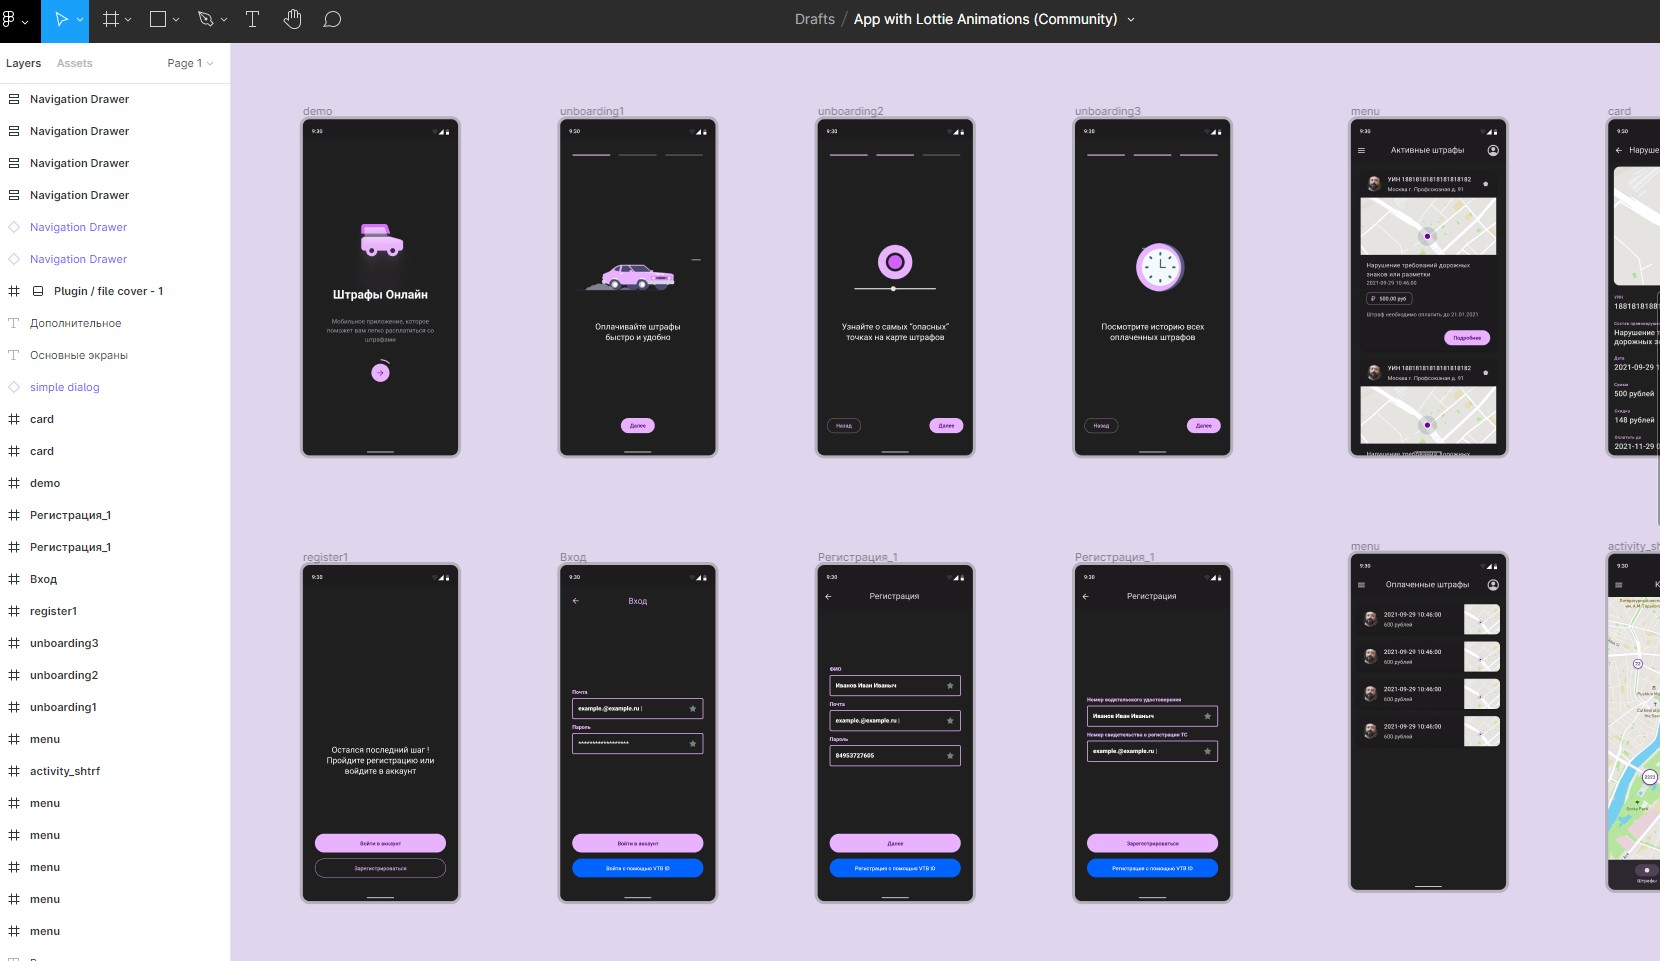
\includegraphics[width=0.7\textwidth]{figuras/figma_exemplo.jpg}
	\fonte{figma.com, 2021}
	\label{fig:figma_exemplo}
\end{figure} 



\subsection{\textit{Node.js}}

O \textit{Node.js} é um ambiente de execução (\textit{runtime}) \textit{Javascript} possibilitando criar aplicações sem depender de um \textit{browser} para a execução. Por meio desta tecnologia, se torna possível empregar o \textit{Javascript} para executar comandos em terminal assim como utilizá-lo para programar qualquer tipo de aplicação \textit{backend} com auxílio de inúmeras bibliotecas desenvolvidas. As bibliotecas do \textit{Node.js} podem ser acessadas e instaladas por seu gerenciador de pacote oficial, o \textit{Node Package Manager} - \textbf{NPM} \cite{NodeJs}.


\subsection{\textit{Electron}}

O \textit{Electron} é um \textit{framework} multiplataforma (Windows, Linux e MacOS) para criação de interfaces possibilitando o usuário acessar serviços do sistema operacional tanto via linha de comando - \textit{CLI} e interface gráfica - \textit{GUI} \cite{Electron}.

\begin{figure}[H]
	\centering
	\caption{Aplicações que utilizam \textit{Electron}}
	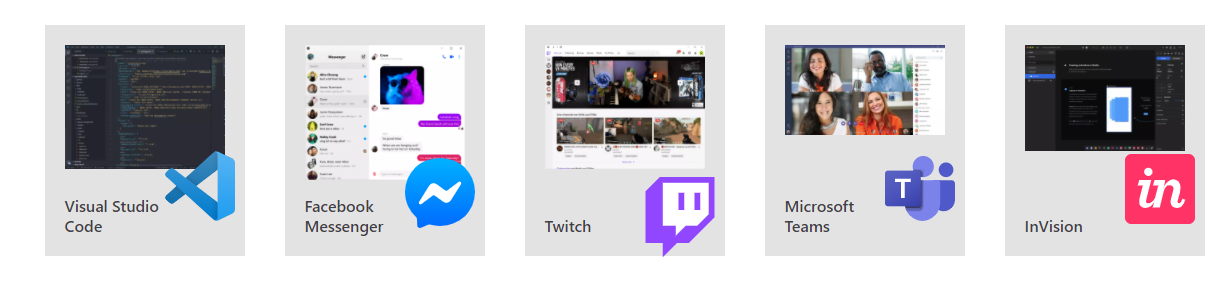
\includegraphics[width=1.0\textwidth]{figuras/electron_apps.png}
	\fonte{Adaptado (electronjs.org, 2020)}
	\label{fig:electron_apps}
\end{figure} 

Por meio dele podemos desenvolver aplicações \textit{desktop} utilizando \textit{HTML}, \textit{CSS}, \textit{Javascript} em conjunto com todas as ferramentas aplicadas a um desenvolvimento \textit{frontend web}. Incorporando o \textit{Chromium}, navegador de código aberto \cite{Chromium}, e \textit{Node.js} no seu binário, toda a base de código fica por conta do \textit{JavaScript} eliminando a experiência de desenvolvimento nativo.

Uma aplicação \textit{Electron} tem como base os seguintes arquivos:

\begin{itemize}
	\item \textbf{\textit{package.json}}: Aponta para o arquivo principal do aplicativo e lista seus detalhes e dependências;
	\item \textbf{\textit{main.js}}: Inicia a aplicação e cria a janela de visualização possibilitando diversas configurações; 
	\item \textbf{\textit{index.html}}: O ponto de partida para a renderização.
\end{itemize}



\subsection{\textit{React}}

O \textit{React} é uma biblioteca \textit{JavaScript}, desenvolvida pela equipe do \textit{Facebook}, que possui ferramentas que facilitam a construção de Interfaces na \textit{Web}. Ele transforma um ambiente complexo, cheio de \textit{Edge Cases} (casos onde você precisa tratar eventos e como os dados são manipulados) em algo muito mais simplificado \cite{React}.

Trabalhando no contexto declarativo, essa biblioteca permite criar telas para cada estado da aplicação, atualizando e renderizando apenas os itens necessários de forma eficiente. Os itens podem ser componentes (arquivos \textit{JSX}) encapsulados que gerenciam seu próprio estado.

\textit{JSX} é uma forma de criar elementos para serem utilizadas como \textit{templates} de aplicações \textit{React}. São bem similares ao código \textit{HTML}, porém, não é interpretado pelo navegador. Por este motivo, deve-se utilizar um transpilador \footnote{\textbf{transpilador}: subconjunto de compiladores os quais identificam um arquivo de código-fonte e o convertem em outro arquivo de código-fonte, sendo de outra linguagem ou em uma versão diferente da mesma linguagem.} para essa conversão. Atualmente, o mais conhecido deles é o \textit{Babel}.

\begin{figure}[H]
	\centering
	\caption{Exemplo de componente \textit{React}}
	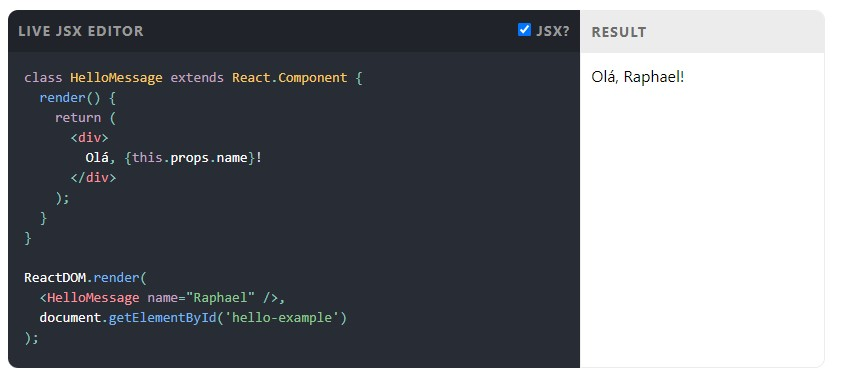
\includegraphics[width=0.8\textwidth]{figuras/exemplo_react.jpg}
	\fonte{Adaptado (reactjs.org, 2021)}
	\label{fig:react_code}
\end{figure} 


\subsection{\textit{React Native}}

Baseado no \textit{React}, para desenvolvimento \textit{WEB}, o \textit{React Native} é um \textit{framework} de codigo aberto desenvolvido pela equipe do \textit{Facebook} que suporta a criação de aplicativos \textit{mobile} multiplataforma (Android e iOS), sem que haja a preocupação de lidar com as linguagens padrões como \textit{Java} ou \textit{Swift}, usando apenas \textit{Javascript}. Como ponto positivo, ao contrário de outros \textit{frameworks} com o mesmo propósito, todo código desenvolvido com \textit{React Native} será convertido para a linguagem nativa do sistema operacional, o que torna a aplicação mais rápida.

\begin{figure}[H]
	\centering
	\caption{Exemplos de \textit{Templates} produzidos com \textit{React Native}}
	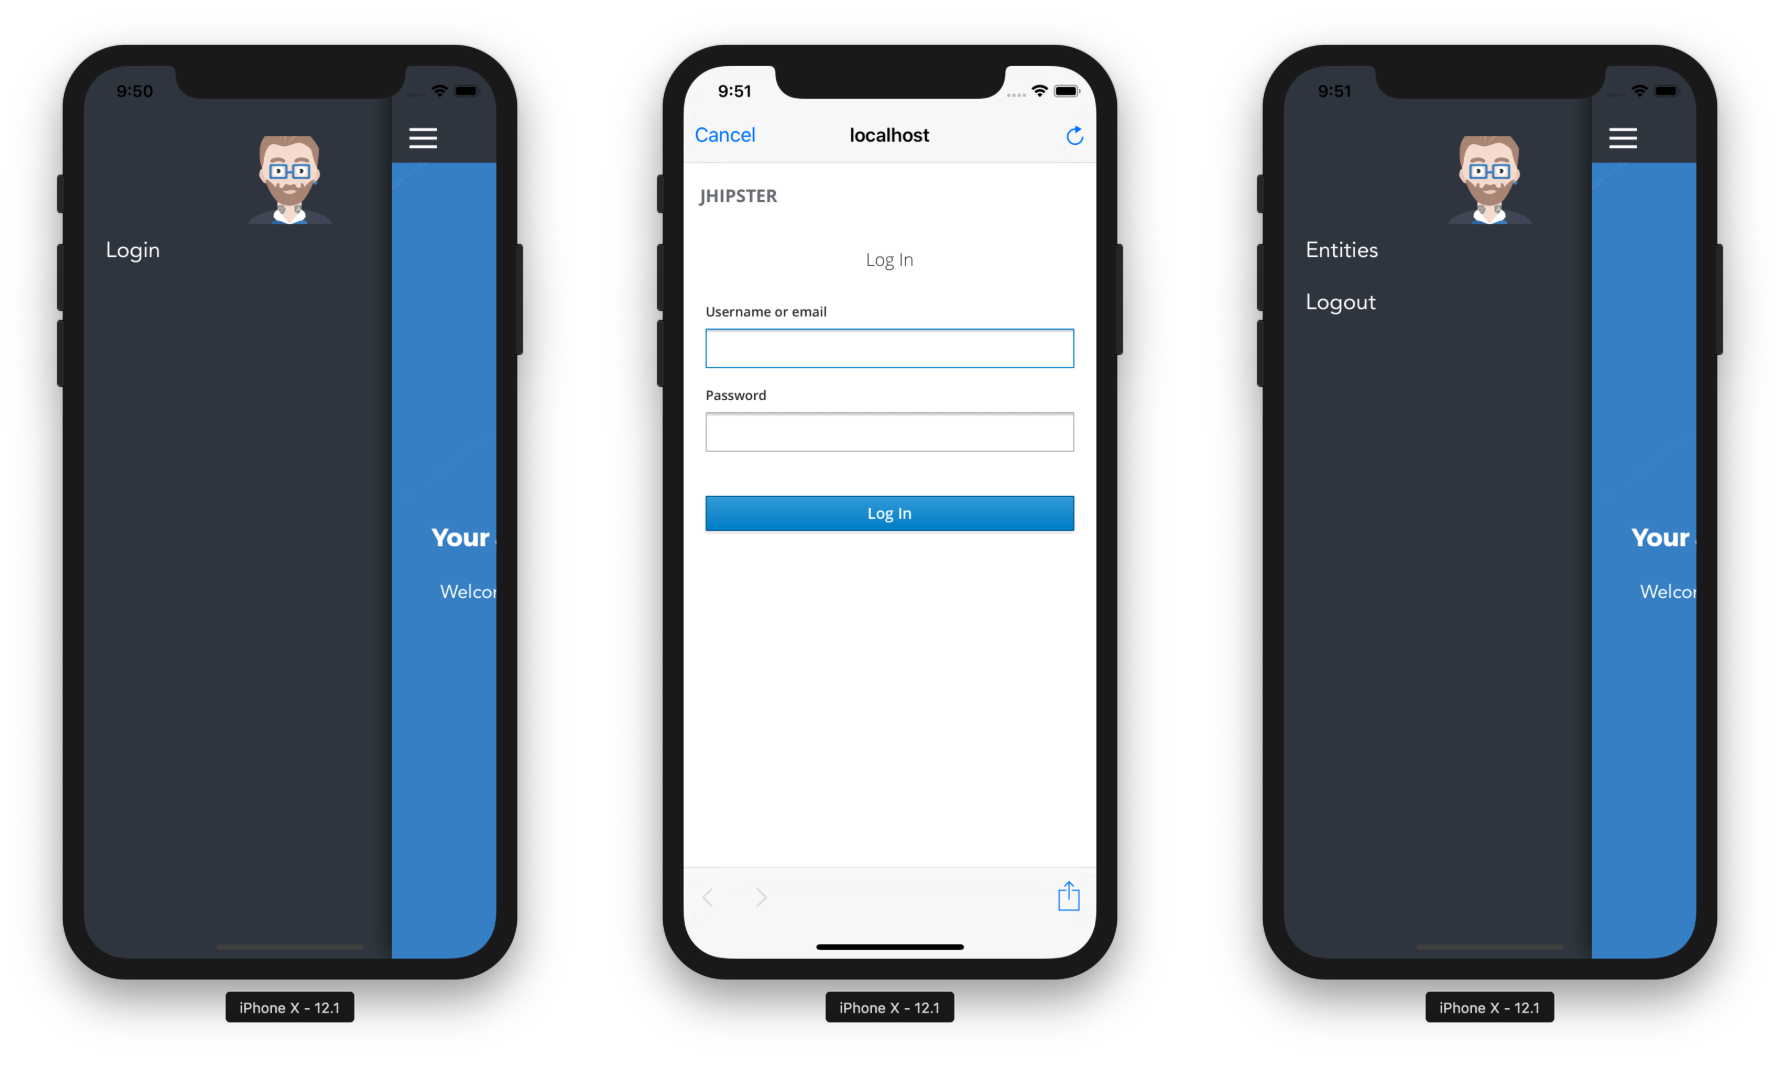
\includegraphics[width=0.7\textwidth]{figuras/react_native_elements.png}
	\fonte{Adaptado (developer.oka, 2021)}
	\label{fig:react-native}
\end{figure} 


	% METODOLOGIA------------------------------------------------------------------

\chapter{METODOLOGIA}
\label{chap:metodologia}


\section{Análise e definição das características do projeto}

Para a metodologia deste trabalho de conclusão de curso, partiu-se do princípio de uma estrutura previamente construída, demostrada no esquema abaixo. A partir dos elementos dessa figura, evidenciados na \autoref{tab:tabela_esquema_cisterna}, foi possível realizar uma análise sobre o que pode ser automatizado, levando em consideração as variáveis e características do sistema.  

\begin{figure}[H]
	\centering
	\caption{Esquema de demonstração de uma cisterna no subsolo}
	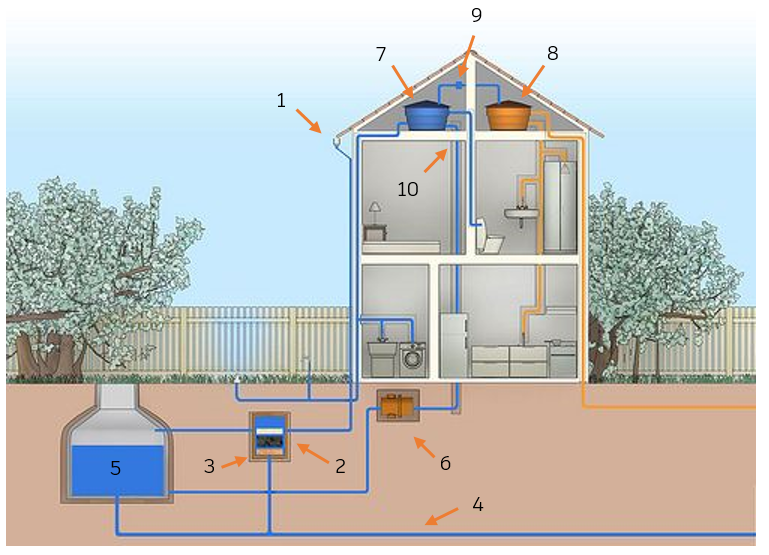
\includegraphics[width=1.0\textwidth]{figuras/esquema_cisterna.png}
	\fonte{Adaptado (ECOMONTES, 2016)}
	\label{fig:esquema_cisterna}
\end{figure}

\newpage

\begin{table}[]
	\centering
	\small
	\begin{tabular}{c|c|c}
		\hline
		\textbf{Identificador} & \textbf{Elemento} & \textbf{Descrição} \\ \hline
		1 & Calha coletora & \begin{tabular}[c]{@{}c@{}}Elemento convencional para coleta e \\ descarte de água da chuva\end{tabular} \\ \hline
		2 & Filtro A (cascalho fino) & \begin{tabular}[c]{@{}c@{}}Elemento para realização de \\ filtragem de pequenas impurezas\end{tabular} \\ \hline
		3 & Filtro B (cascalho grosso) & \begin{tabular}[c]{@{}c@{}}Elemento para realização de \\ filtragem de impurezas\end{tabular} \\ \hline
		4 & Tubulação de descarte & \begin{tabular}[c]{@{}c@{}}Tubulação utilizada como rota de escoamento \\ quando o reservatório não está em uso ou \\ está cheio\end{tabular} \\ \hline
		5 & Reservatório de coleta & Cisterna propriamente dita \\ \hline
		6 & Motobomba ou bomda d'água & \begin{tabular}[c]{@{}c@{}}Elemento utilizado para realização do \\ ganho de elevação da água\end{tabular} \\ \hline
		7 & Caixa d'água auxiliar & \begin{tabular}[c]{@{}c@{}}Caixa d'água convencional com alimentação \\ oriunda da bomba d'água\end{tabular} \\ \hline
		8 & Caixa d'água convencional & \begin{tabular}[c]{@{}c@{}}Caixa d'água padrão com alimentação \\ da estação de água da cidade\end{tabular} \\ \hline
		9 & Elo de ligação & \begin{tabular}[c]{@{}c@{}}Ligação utilizada para abastecer a caixa d'água \\ auxiliar quando a cisterna está seca \\ ou em manutenção\end{tabular} \\ \hline
		10 & Distribuidor & \begin{tabular}[c]{@{}c@{}}Elementos de distribuição de água \\ para pontos estratégicos\end{tabular} \\ \hline
	\end{tabular}
	\caption{Identificação dos elementos da \autoref{fig:esquema_cisterna}.}
	\label{tab:tabela_esquema_cisterna}
\end{table}
% https://www.tablesgenerator.com

Com base nesses elementos é importante destacar os seguintes pontos para as implementações que serão tratadas nas seções posteriores:

\begin{itemize}
	\item Definir o método ou sistema para medição de nível do item 5;
	\item Elaborar o sistema de ativação/desativação da motobomba do item 6;
	\item Definir o método ou sistema para medição de nível do item 7;
	\item Elaborar um sistema para intermediar/controlar a passagem de água no elo de ligação (item 9);
	\item Definir um sistema para administrar o descarte de água da cisterna (item 4);
	\item Esquematizar e situar os sistemas para envio e aquisição de dados, tornando-se possível realizar remotamente as operações citadas nos itens anteriores; 
	\item Configurar um pequeno servidor para intermediar entre os dispositivos microcontrolados e as interfaces de controle;  
	\item Implementar as interfaces para visualizar/comandar os pontos citados nos itens anteriores.
\end{itemize}

Dois módulos distintos foram propostos: \textbf{\textit{Tank Control Module} - TCM}, o qual será responsável pelo monitoramento e controle da caixa d'água auxiliar (\autoref{fig:esquema_cisterna}, identificador 7) e \textbf{\textit{Cistern Control Module} - CCM}, responsável pelo monitoramento e controle da cisterna (\autoref{fig:esquema_cisterna}, identificador 5). O diagrama da \autoref{fig:esquema_proj} mostra o esquema proposto para a criação do projeto. 

\begin{figure}[H]
	\centering
	\caption{Esquema básico do projeto.}
	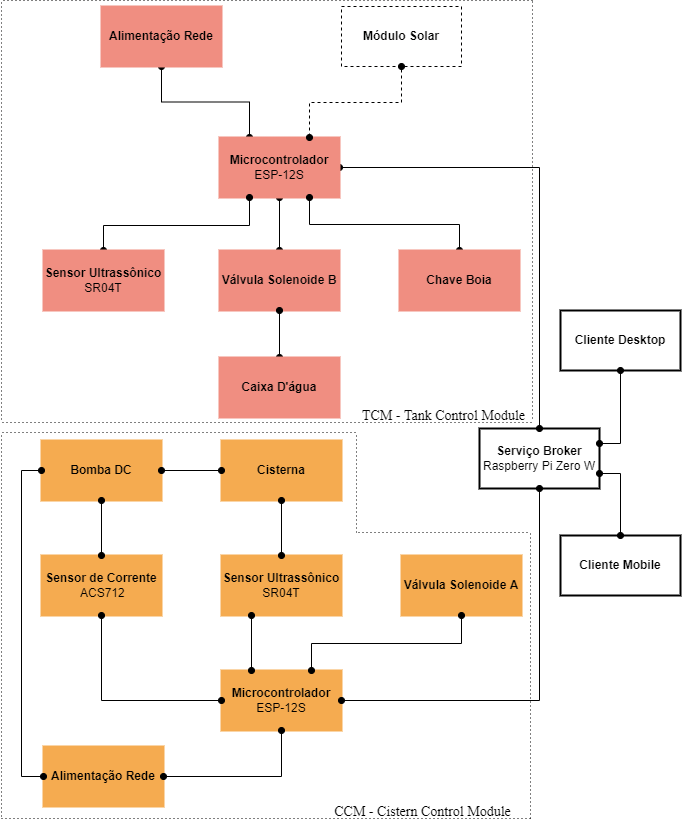
\includegraphics[width=1.05\textwidth]{figuras/esquema_basico_proj_2.png}
	\fonte{Própria}
	\label{fig:esquema_proj}
\end{figure} 

\section{Organização do trabalho}

Iniciou-se com a criação do quadro \textit{Kanban} (\autoref{fig:kanban-proj}), para auxílio da organização das tarefas, e com a criação do repositório no \textit{Github} (\autoref{fig:github}) para armazenamento e versionamento dos códigos das vertentes de \textit{Firmware} e \textit{Software} do projeto. Deu-se prosseguimento com os estudos e levantamentos bibliográficos relacionando três áreas do projeto. Buscou-se encontrar os métodos,  ferramentas, tecnologias, bibliotecas e \textit{frameworks} mais adequados para a implementação do projeto.  Diante de cada seleção feita, foram executadas análises para que fosse definido o funcionamento do sistema total, munido da combinação de cada uma das três áreas citadas anteriormente e visando a geração de um produto que pudesse ser empregado no mercado: atrativo economicamente e seguindo diretrizes sustentáveis.  

Primeiramente, na seção de \textit{hardware}, foram selecionados as ferramentas para modelagem de placas de circuito impresso - \textit{PCB's} e para modelagem de peças \textit{3D}, através de manufatura aditiva, a escolha de todos os dispositivos eletrônicos a serem utilizados e a análise do local de aplicação. Posteriormente, na parte de \textit{firmware}, já estando selecionados os microcontroladores e o microprocessador, foram determinadas todas as rotinas de operação e escolhidas, respectivamente, as linguagens para programá-los e o \textit{framework} para criação de um sistema operacional embarcado baseado em \textit{kernel Linux}. Na parte de \textit{software}, foram selecionadas as ferramentas para a criação de interfaces dentro da camada \textit{front-end}: aplicações \textit{mobile} e \textit{desktop}.

Por fim, elaborou-se a lista de materiais necessários para construção o projeto, tendo objetivo de validação em ambiente real, efetuando testes de longos períodos, averiguando a integridade do sistema, a robustez dos componentes e a identificação de casos não previstos anteriormente, tornando possível a aplicação de melhorias posteriores a entrega deste trabalho.

\begin{figure}[H]
	\centering
	\caption{Visão geral do quadro \textit{Kanban} criado na ferramenta \textit{Trello}}
	\includegraphics[width=0.85\textwidth]{figuras/visão_geral_meu_kanban.png}
	\fonte{Própria.}
	\label{fig:kanban-proj}
\end{figure}


\begin{figure}[H]
	\centering
	\caption{Visão geral repositório criado no \textit{Github}}
	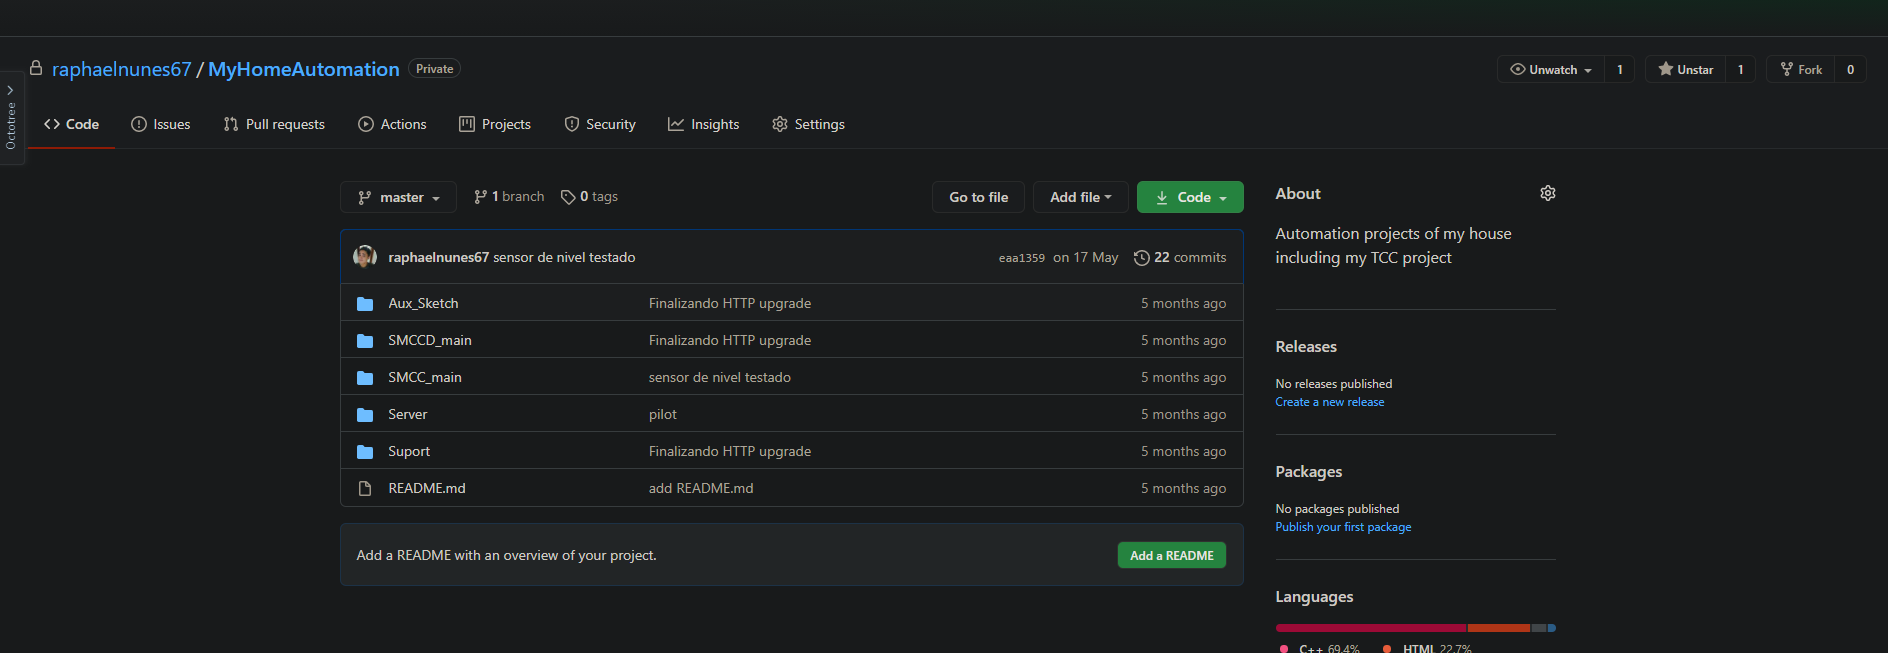
\includegraphics[width=0.85\textwidth]{figuras/github.png}
	\fonte{Própria.}
	\label{fig:github}
\end{figure}



\section{Levantamento do referencial bibliográfico e capacitação}
\label{sec:metmodal}

Essa parte do trabalho conteve-se no levantamento de referências bibliográficas relacionadas com os temas de \textit{IoT}, programação de microcontroladores, criação de aplicações com \textit{frameworks} baseados em \textit{Javascript}. Também buscou-se a capacitação em cursos oferecidos pelas plataformas \textit{Alura}, \textit{Udemy} e \textit{Skylab (Rocketseat)} o aprendizado de conteúdos complementares ao curso de formação em engenheria de controle e automação, como a criação de placas de circuito impresso, treinamentos sobre \textit{Linux} embarcado, implementação do protocolo \textit{MQTT}, criação de \textit{APPs Android} com \textit{React Native} e aplicações \textit{Desktop} com \textit{Electron.js}.

\section{Desenvolvimento dos elementos de \textit{Hardware}}
\label{sec: dev_ele_hw}

Nesse momento foram definidos todos os elementos de \textit{hardware} necessários para a execução do projeto: para os dispositivos eletrônicos, documentos como \textit{Datasheets}, catálogos e informativos de dispositivos elétricos foram coletados para consulta durante o decorrer do trabalho; para a parte estrutural executou-se a enumeração de peças que deveriam o desenhadas com auxílio do \textit{Software Autodesk Inventor} e posteriormente construídas através de manufatura aditiva.  Realizou-se uma busca no mercado pelos componentes necessários efetuando as possíveis compras e elaborando o orçamento geral do projeto.

\subsection{O circuito de alimentação}

Nesta etapa do projeto iniciou-se a criação do circuito de alimentação para os módulos \textbf{CCM} e \textbf{TCM}. Partindo-se da fonte chaveada definida no \autoref{chap:fundamentacao-teorica}, a qual transforma 110V AC em 12V DC, criou-se um conversor DC-DC do tipo \textit{Buck} para converter a tensão de saída da fonte para 3.3V, ideais para alimentação dos sensores e microcontroladores. 

\begin{figure}[H]
	\centering
	\caption{Esquma de ligação do circuito de alimentação}
	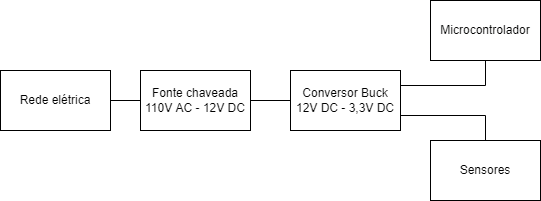
\includegraphics[width=0.8\textwidth]{figuras/alimentacao.png}
	\fonte{Própria.}
	\label{fig:alimentacao_esquema}
\end{figure}

Após a definição do esquema de medição, procurou-se dimensionar o conversor \textit{Buck}. O dimensionamento deu-se a partir das leituras dos \textit{datasheets} de todos os dispositivos que futuramente poderiam ser utilizados. Outro ponto importante salientar para a escolha do conversor \textit{Buck} foi a disponibilidade no mercado.

Dentre os fatores citados o conversor selecionado foi o LM2596, o qual podemos encontrar um módulo com sua aplicação típica (\autoref{fig:conversor_buck}) com certa facilidade no mercado. A \autoref{fig:conversor_buck_teste} mostra o teste realizado em bancada.

\begin{figure}[H]
	\centering
	\caption{Aplicação típica do LM2596.}
	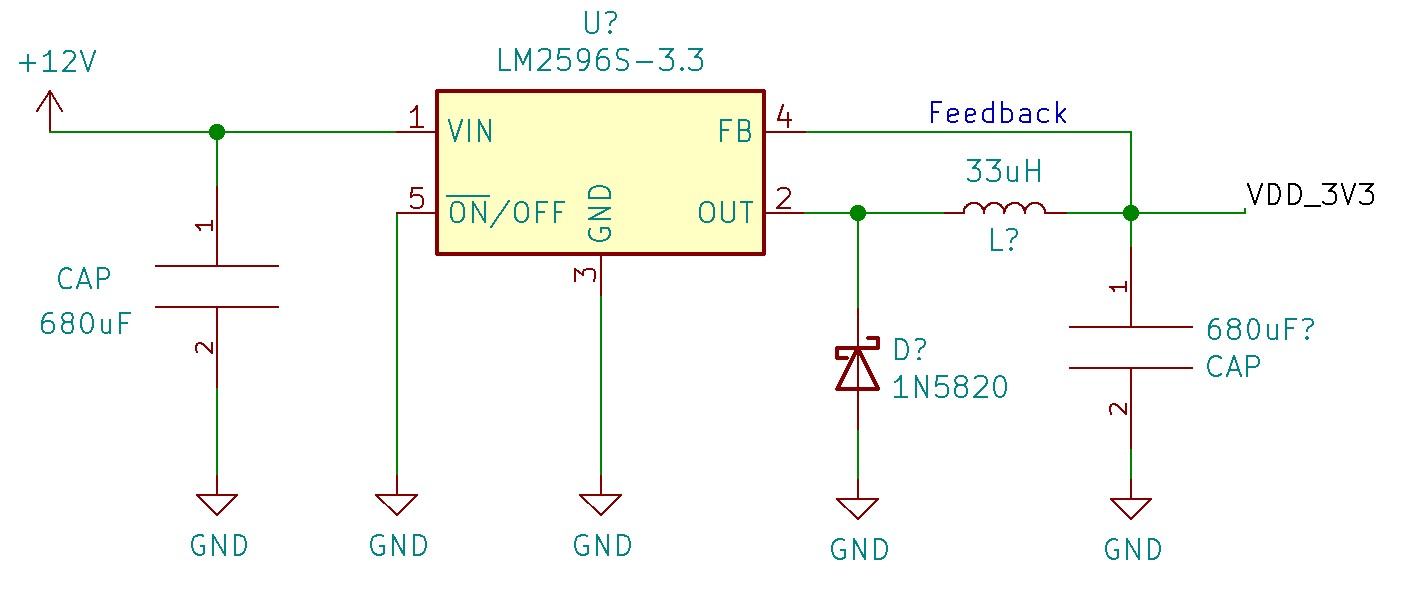
\includegraphics[width=0.8\textwidth]{figuras/conversor_buck.jpg}
	\fonte{Própria.}
	\label{fig:conversor_buck}
\end{figure}

\begin{figure}[H]
	\centering
	\caption{Teste em bancada do módulo com LM2596.}
	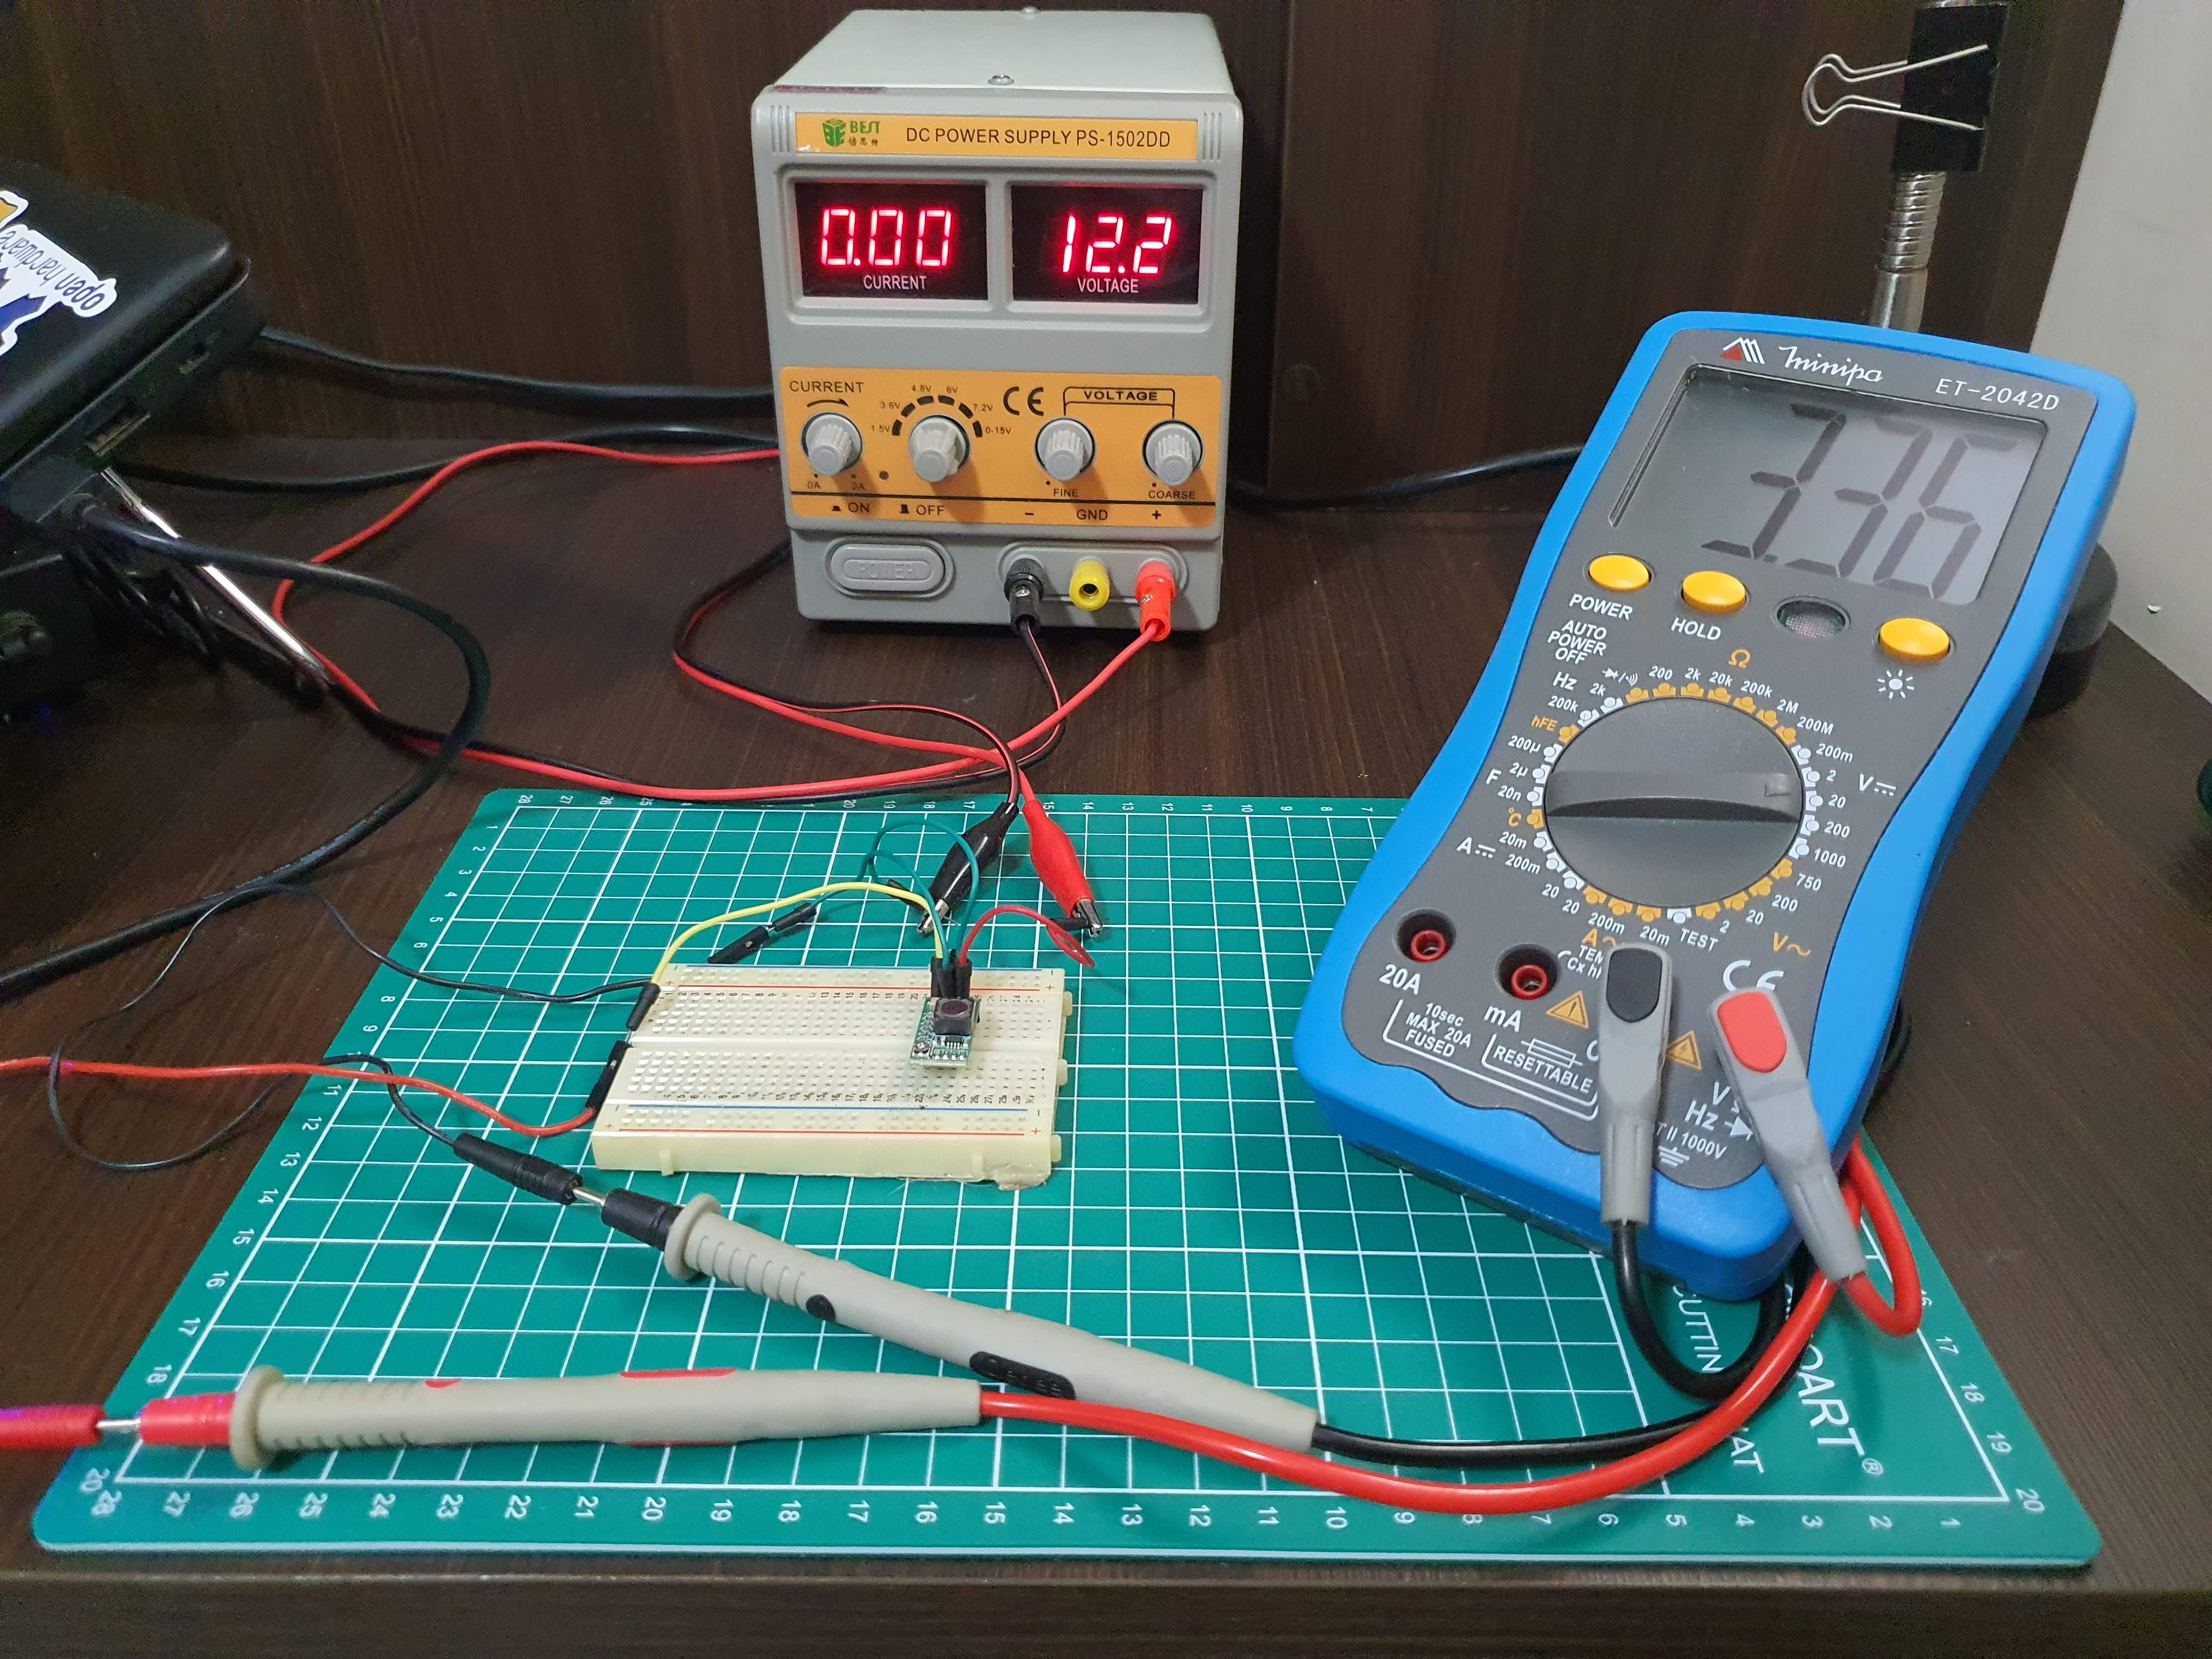
\includegraphics[width=0.7\textwidth]{figuras/conversor_buck_teste.jpg}
	\fonte{Própria.}
	\label{fig:conversor_buck_teste}
\end{figure}

\subsection{O circuito de detecção de fechadura da chave}
\subsection{O circuito de medição de nível}
\subsection{O circuito de ativação da motobomba}
\subsection{O circuito de ativação da válvula}

\section{Desenvolvimento dos elementos de \textit{Firmware}}
\label{sec: dev_ele_fw}

A definição e desenvolvimento dos elementos de \textit{Firmware} se deu após todos os levantamentos de requisitos do trabalho. Esse momento concentrou-se na escolha de tecnologias mais fáceis de implementação, que tivessem uma gama de documentações e que fossem empregadas em produtos oficiais. Para lidar com o uso dos microprocessadores e microcontroladores, foram feitas pesquisas visando consolidar conceitos aprendidos durante o curso de graduação.

\subsection {Instalação e configuração do \textit{Broker MQTT}}
\subsection {Programação do servidor}
\subsection {Definição de utilização dos pinos do ESP-12S}
\subsection{Organização dos arquivos internos dos microcontroladores}
\subsection {Implementação do \textit{Driver WIFI}}
\subsection {Implementação do \textit{Driver MQTT}}
\subsection{Implementação da rotina de Reset}
\subsection{Implementação da funcionalidade de \textit{ OTA Upgrade}}
\subsection{Implementação do modo de \textit{DeepSleep}}


\section{Desenvolvimento dos elementos de \textit{Software}}


Para o desenvolvimento dos elementos de \textit{Software} buscou-se a participação de cursos básicos e avançados sobre aplicações \textit{front-end}, as quais servem de conteúdo complementar aos temas abordados na graduação em engenharia de controle e automação.

Os cursos adquiridos trouxeram uma série de conhecimentos para uma maior interação entre desenvolvedor e usuário, possibilitando a criação de interfaces intuitivas e agregando novas informações e visões a outros temas, como na programação de sistemas embarcados.

\section{Desenvolvimento da aplicação \textit{Desktop}}
\section{Desenvolvimento da aplicação \textit{Mobile}}



\subsection{Os elementos de ativação e desativação}

Tendo em vista os elementos descritos nos itens anteriores, tornou-se necessário a implementação de um circuito para ativação e desativação da bomba d'água assim como a execução de técnicas de proteção e isolamento.

O diagrama desenvolvido no \textit{software Proteus} (\autoref{fig:diagramaproteus}) mostra a integração de como seria o sistema de ativação e desativação da motobomba.

\begin{figure}[H]
	\centering
	\caption{Diagrama de ativação com partida lenta}
	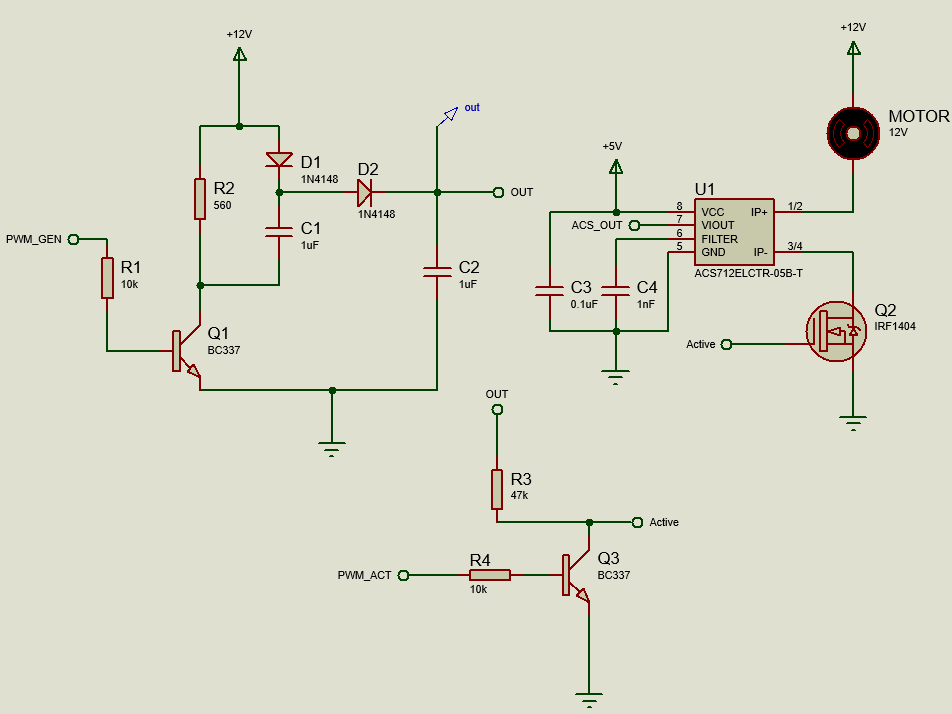
\includegraphics[width=0.9\textwidth]{figuras/diagrama_ativação_bomba.png}
	\fonte{Própria}
	\label{fig:diagramaproteus}
\end{figure} 

A partir deste diagrama utilizou-se técnicas de partida lenta através do chaveamento transistorizado (\textit{BC546}). Por meio do \textit{PWM - Pulse-Width Modulation} oriundo do microcontrolador, o transistor realiza a alteração sobre o valor eficaz de tensão aplicada na bomba d'água.

Para saturação do transistor \textit{IRF1404} (\autoref{fig:IRF1404}) foi desenvolvido o circuito dobrador de tensão também evidenciado na \autoref{fig:diagramaproteus}. A ideia desse circuito é garantir uma queda de tensão entre \textit{GATE} e \textit{SOURCE} duas vezes maior (em torno de \textit{24V}) que a tensão de alimentação do circuito.

\begin{figure}[H]
	\centering
	\caption{Transistor IRF1404}
	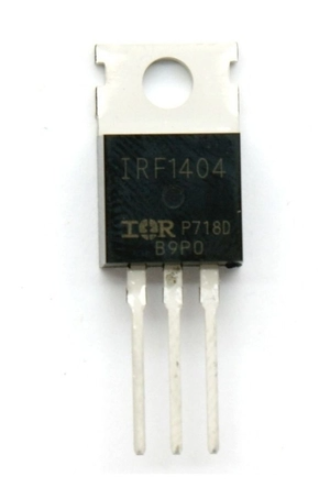
\includegraphics[width=0.2\textwidth]{figuras/IRF1404.png}
	\fonte{ALLDATASHEET, 2020}
	\label{fig:IRF1404}
\end{figure} 

	% CRONOGRAMA------------------------------------------------------------------

\chapter{CRONOGRAMA}
\label{chap:cronograma}

 \begin{figure}[H]
 	\centering
 	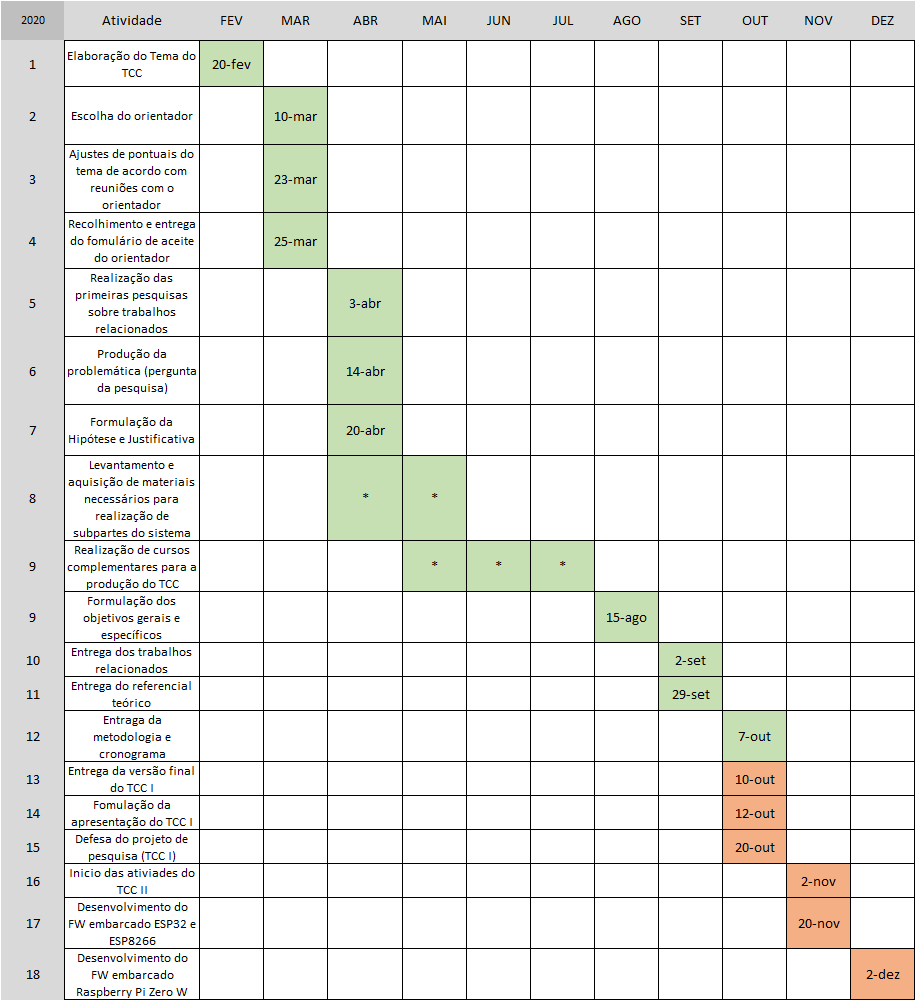
\includegraphics[width=1.0\textwidth]{tabelas/cronograma_2020.png}
 	\caption*{Representação das atividades desenvolvidas no ano de 2020.}
 \end{figure}
 \newpage
  \begin{figure}[H]
 	\centering
 	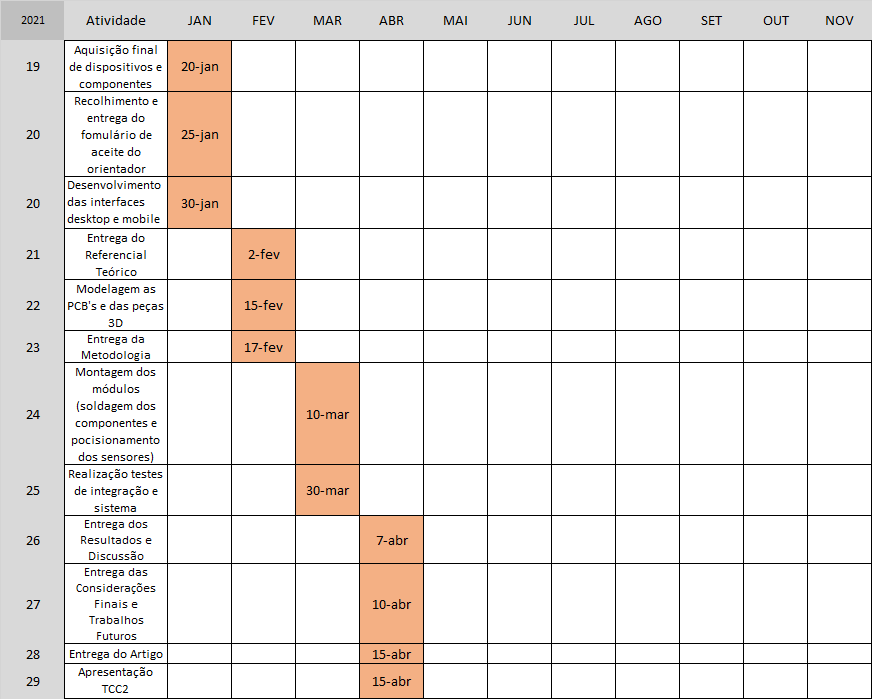
\includegraphics[width=1.0\textwidth]{tabelas/cronograma_2021.png}
 	\caption*{Representação das atividades desenvolvidas no ano de 2021.}
 \end{figure}
	%% RESULTADOS-------------------------------------------------------------------

\chapter{RESULTADOS}
\label{chap:resultados}

%Cada capítulo deve conter uma pequena introdução (tipicamente, um ou dois parágrafos) que deve deixar claro o objetivo e o que será discutido no capítulo, bem como a organização do capítulo. 

\section{Análise modal numérica}
\label{sec:resultmodal}

Na análise modal, as frequências naturais obtidas para os dois casos mantiveram-se afastadas da faixa de operação da turbina. Considerando uma TSR entre 2 e 3,5 e uma faixa de velocidade comumente encontrada entre 1 e 2 $m/s$ tem-se uma faixa de frequências de operação variando entre 0,62 e 2,16 $Hz$ que se encontra distante das frequências naturais encontradas para os casos analisados conforme apresentado na \autoref{tab:resultfreqturbina}. Tal verificação vem confirmar a possibilidade de utilização da consideração de 1 GDL. 

\begin{table}[h]
	\centering
	\caption{Frequências naturais obtidas [Hz].}
	\label{tab:resultfreqturbina}	
	    \begin{tabular}{c c c}
        \hline Modo &  &  \\
         & Maciço & Tubo \\
        \hline        
		1 & 9,04 & 7,54 \\
		2 & 9,08 & 7,55 \\
		3 & 13,40 & 9,80 \\
		4 & 28,68 & 20,19\\
		5 & 28,74 & 20,21 \\
		6 & 30,32 & 24,56 \\
		\hline
    \end{tabular}

	\fonte{Autoria própria.}
\end{table}

As \autoref{fig:resultmodomacico} e \autoref{fig:resultmodotubos} apresentam algumas respostas esperadas para o primeiro e sexto modo de vibração. Nelas é possível verificar a importância da verificação das frequências de operação da turbina, que caso negligenciado pode levar a sérios danos. Também pode-se verificar que a utilização do tubo em comparação aos eixos maciços levaram a maiores deformações.    

\begin{figure}	
	\caption{Modos de vibração do sistema com eixo e braço maciços.}
	\label{fig:resultmodomacico}
	\begin{subfigure}{0.5\textwidth}
		\centering
		\includegraphics[width=1.0\textwidth]{figuras/resultmodalmacico1.pdf}
		\caption{Primeiro modo.}
		\label{subfig:resultmodomacicomodo1}
	\end{subfigure}
	\begin{subfigure}{0.5\textwidth}
		\centering
		\includegraphics[width=0.95\textwidth]{figuras/resultmodalmacico6.pdf}
		\caption{Sexto modo.}
		\label{subfig:resultmodomacicomodo6}
	\end{subfigure}		
	\fonte{Autoria própria.}
\end{figure}


\section{Double-multiple streamtube model}
\label{sec:resultdmsm}

Em termos de torque, a \autoref{fig:resultCtPaFrontPost} apresenta o gráfico da coeficiente de torque para uma pá, onde é possível verificar que uma maior quantidade de torque é extraído no primeiro meio ciclo (0 - 180 graus) quando comparado com o segundo (180 - 360 graus).

\begin{figure}
	\centering
	\caption{Coeficiente de torque para uma pá.}
	\includegraphics[width=0.8\textwidth]{figuras/resultCtPaFrontPost.eps}
	\fonte{Autoria própria.}
	\label{fig:resultCtPaFrontPost}
\end{figure}

\section{Próximas etapas}
\label{sec:trabalhosFuturos}

Os próximos passos a serem feitos estão sintetizados na \autoref{tab:cronograma}.

\begin{table}[H]
	\centering
	\caption{Cronograma.}
	\label{tab:cronograma}
	    \begin{tabular}{l c c c c c c}
        \hline TAREFA & SEM 1 & SEM 2 & SEM 3 & SEM 4 & SEM 5 & SEM 6\\
        \hline        
		Verificação da influencia da água & X & & & & & \\
		Acoplamento trem de potência & X & X & X & & & \\
		Elaboração e submissão de artigo & & & X & X & X &\\
		Redação final & X& X& X& X & X & X\\
		Submissão de versão final & & & & & & X \\
		\hline
    \end{tabular}

	\fonte{Autoria Própria.}
\end{table}

\begin{quadro}[!htb]
	\centering
	\caption{Exemplo de Quadro.\label{qua:quadro-exemplo1}}
	\begin{tabular}{|p{7cm}|p{7cm}|}
		\hline
		\textbf{BD Relacionais} & \textbf{BD Orientados a Objetos} \\
		\hline
		Os dados são passivos, ou seja, certas operações limitadas podem ser automaticamente acionadas quando os dados são usados. Os dados são ativos, ou seja, as solicitações fazem com que os objetos executem seus métodos. & Os processos que usam dados mudam constantemente. \\
		\hline
	\end{tabular}
	\fonte{XXXXXXXXXXXX.}
\end{quadro}
	%% ORIENTAÇÕES GERAIS------------------------------------------------------------


% SOBRE AS ILUSTRAÇÕES----------------------------------------------------------
\chapter{SOBRE AS ILUSTRAÇÕES}
\label{chap:apSobreIlust}

A seguir exemplifica-se como inserir ilustrações no corpo do trabalho. As ilustrações serão indexadas automaticamente em suas respectivas listas. A numeração sequencial de figuras, tabelas e equações também ocorre de modo automático.

Referências cruzadas são obtidas através dos comandos \verb|\label{}| e \verb|\ref{}|. Sendo assim, não é necessário por exemplo, saber que o número de certo capítulo é \ref{chap:fundamentacaoTeorica} para colocar o seu número no texto. Outra forma que pode ser utilizada é esta: \autoref{chap:fundamentacaoTeorica}, facilitando a inserção, remoção e manejo de elementos numerados no texto sem a necessidade de renumerar todos esses elementos.

% FIGURAS-----------------------------------------------------------------------
\chapter{FIGURAS}
\label{chap:figuras}

Exemplo de como inserir uma figura. A \autoref{fig:figura-exemplo1} aparece automaticamente na lista de figuras. Para saber mais sobre o uso de imagens no \LaTeX{} consulte literatura especializada \cite{Goossens2007}.

Os arquivos das figuras devem ser armazenados no diretório de "/dados".

\begin{figure}[!htb]
    \centering
    \caption{Exemplo de Figura}
    \includegraphics[width=0.5\textwidth]{./dados/figuras/figura1}
    \fonte{\citeonline{IRL2014}}
    \label{fig:figura-exemplo1}
\end{figure}

% QUADROS E TABELAS---------------------------------------------------------------
\chapter{QUADROS E TABELAS}
\label{chap:tabelas}

Exemplo de como inserir o \autoref{qua:quadro-exemplo1} e a \autoref{tab:tabela-exemplo1}. Ambos aparecem automaticamente nas suas respectivas listas. Para saber mais informações sobre a construção de tabelas no \LaTeX{} consulte literatura especializada \cite{Mittelbach2004}.

Ambos os elementos (Quadros e Tabelas) devem ser criados em arquivos separados para facilitar manutenção e armazenados no diretório de "/dados".

\input{./dados/quadros/quadro1}

A diferença entre quadro e tabela está no fato que um quadro é formado por linhas horizontais e verticais. Deve ser utilizado quando o conteúdo é majoritariamente não-numérico. O número do quadro e o título vem acima do quadro, e a fonte, deve vir abaixo. E Uma tabela é formada apenas por linhas verticais. Deve ser utilizada quando o conteúdo é majoritariamente numérico. O número da tabela e o título vem acima da tabela, e a fonte, deve vir abaixo, tal como no quadro.

\begin{table}[!htb]
    \centering
    \caption[Resultado dos testes]{Resultado dos testes.
    \label{tab:tabela-exemplo1}}
    \begin{tabular}{rrrrr}
        \toprule
            & Valores 1 & Valores 2 & Valores 3 & Valores 4 \\
        \midrule
            Caso 1 & 0,86 & 0,77 & 0,81 & 163 \\
            Caso 2 & 0,19 & 0,74 & 0,25 & 180 \\
            Caso 3 & 1,00 & 1,00 & 1,00 & 170 \\
        \bottomrule
    \end{tabular}
    \fonte{XXXXXXXX}
\end{table}


% EQUAÇÕES-----------------------------------------------------------------------
\chapter{EQUAÇÕES}
\label{chap:equacoes}

Exemplo de como inserir a \autoref{eq:equacao-exemplo1} e a Eq. \ref{eq:equacao-exemplo2} no corpo do texto \footnote{Deve-se atentar ao fato de a formatação das equações ficar muito boa esteticamente.}. Observe que foram utilizadas duas formas distintas para referenciar as equações.

\begin{equation}
    X(s) = \int\limits_{t = -\infty}^{\infty} x(t) \, \text{e}^{-st} \, dt
    \label{eq:equacao-exemplo1}
\end{equation}

\begin{equation}
    F(u, v) = \sum_{m = 0}^{M - 1} \sum_{n = 0}^{N - 1} f(m, n) \exp \left[ -j 2 \pi \left( \frac{u m}{M} + \frac{v n}{N} \right) \right]
    \label{eq:equacao-exemplo2}
\end{equation}

% ALGORITMOS-----------------------------------------------------------------------
\chapter{ALGORITMOS}
\label{chap:algoritmos}

Exemplo de como inserir um algoritmo. Para inserção de algoritmos utiliza-se o pacote {\ttfamily algorithm2e} que já está devidamente configurado dentro do template.

Os algoritmos devem ser criados em arquivos separados para facilitar manutenção e armazenados no diretório de "/dados".\\
\\

\input{./dados/algoritmos/algoritmo1}

% SOBRE AS LISTAS--------------------------------------------------------------------
\chapter{SOBRE AS LISTAS}
\label{chap:apSobreLista}

Para construir listas de "\textit{bullets}"{} ou listas enumeradas, inclusive listas aninhadas, é utilizado o pacote \verb|paralist|.

Exemplo de duas listas não numeradas aninhadas, utilizando o comando \verb|\itemize|. Observe a indentação, bem como a mudança automática do tipo de "\textit{bullet}"{} nas listas aninhadas.

\begin{itemize}
    \item item não numerado 1
    \item item não numerado 2
    \begin{itemize}
        \item subitem não numerado 1
        \item subitem não numerado 2
        \item subitem não numerado 3
    \end{itemize}
    \item item não numerado 3
\end{itemize}

Exemplo de duas listas numeradas aninhadas, utilizando o comando \verb|\enumerate|. Observe a numeração progressiva e indentação das listas aninhadas.

\begin{enumerate}
    \item item numerado 1
    \item item numerado 2
    \begin{enumerate}
        \item subitem numerado 1
        \item subitem numerado 2
        \item subitem numerado 3
    \end{enumerate}
    \item item numerado 3
\end{enumerate}

% SOBRE AS CITAÇÕES E CHAMADAS DE REFERÊNCAS----------------------------------------------
\chapter{SOBRE AS CITAÇÕES E CHAMADAS DE REFERÊNCAS}
\label{chap:apSobreCita}

Citações são trechos de texto ou informações obtidas de materiais consultadss quando da elaboração do trabalho. São utilizadas no texto com o propósito de esclarecer, completar e embasar as ideias do autor. Todas as publicações consultadas e utilizadas (por meio de citações) devem ser listadas, obrigatoriamente, nas referências bibliográficas, para preservar os direitos autorais. São classificadas em citações indiretas e diretas.

% CITAÇÕES INDIRETAS-----------------------------------------------------------------------
\chapter{CITAÇÕES INDIRETAS}
\label{chap:citacoesLivres}

É a transcrição, com suas próprias palavras, das idéias de um autor, mantendo-se o sentido original. A citação indireta é a maneira que o pesquisador tem de ler, compreender e gerar conhecimento a partir do conhecimento de outros autores. Quanto à chamada da referência, ela pode ser feita de duas maneiras distintas, conforme o nome do(s) autor(es) façam parte do seu texto ou não. Exemplo de chamada fazendo parte do texto:\\
\\Enquanto \citeonline{Maturana2003} defendem uma epistemologia baseada na biologia. Para os autores, é necessário rever \ldots.\\

A chamada de referência foi feita com o comando \verb|\citeonline{chave}|, que produzirá a formatação correta.

A segunda forma de fazer uma chamada de referência deve ser utilizada quando se quer evitar uma interrupção na sequência do texto, o que poderia, eventualmente, prejudicar a leitura. Assim, a citação é feita e imediatamente após a obra referenciada deve ser colocada entre parênteses. Porém, neste caso específico, o nome do autor deve vir em caixa alta, seguido do ano da publicação. Exemplo de chamada não fazendo parte do texto:\\
\\Há defensores da epistemologia baseada na biologia que argumentam em favor da necessidade de \ldots \cite{Maturana2003}.\\

Nesse caso a chamada de referência deve ser feita com o comando \verb|\cite{chave}|, que produzirá a formatação correta.

% CITAÇÕES DIRETAS-----------------------------------------------------------------------
\chapter{CITAÇÕES DIRETAS}
\label{chap:citacoesLiterais}

É a transcrição ou cópia de um parágrafo, de uma frase, de parte dela ou de uma expressão, usando exatamente as mesmas palavras adotadas pelo autor do trabalho consultado.

Quanto à chamada da referência, ela pode ser feita de qualquer das duas maneiras já mencionadas nas citações indiretas, conforme o nome do(s) autor(es) façam parte do texto ou não. Há duas maneiras distintas de se fazer uma citação direta, conforme o trecho citado seja longo ou curto.

Quando o trecho citado é longo (4 ou mais linhas) deve-se usar um parágrafo específico para a citação, na forma de um texto recuado (4 cm da margem esquerda), com tamanho de letra menor e espaçamento entrelinhas simples. Exemplo de citação longa:
\\\begin{citacao}
    Desse modo, opera-se uma ruptura decisiva entre a reflexividade filosófica, isto é a possibilidade do sujeito de pensar e de refletir, e a objetividade científica. Encontramo-nos num ponto em que o conhecimento científico está sem consciência. Sem consciência moral, sem consciência reflexiva e também subjetiva. Cada vez mais o desenvolvimento extraordinário do conhecimento científico vai tornar menos praticável a própria possibilidade de reflexão do sujeito sobre a sua pesquisa \cite[p.~28]{Silva2000}.
\end{citacao}

Para fazer a citação longa deve-se utilizar os seguintes comandos:
\begin{verbatim}
\begin{citacao}
<texto da citacao>
\end{citacao}
\end{verbatim}

No exemplo acima, para a chamada da referência o comando \verb|\cite[p.~28]{Silva2000}| foi utilizado, visto que os nomes dos autores não são parte do trecho citado. É necessário também indicar o número da página da obra citada que contém o trecho citado.

Quando o trecho citado é curto (3 ou menos linhas) ele deve inserido diretamente no texto entre aspas. Exemplos de citação curta:\\
\\A epistemologia baseada na biologia parte do princípio de que "assumo que não posso fazer referência a entidades independentes de mim para construir meu explicar" \cite[p.~35]{Maturana2003}.\\
\\A epistemologia baseada na biologia de \citeonline[p.~35]{Maturana2003} parte do princípio de que "assumo que não posso fazer referência a entidades independentes de mim para construir meu explicar".

% DETALHES SOBRE AS CHAMADAS DE REFERÊNCIAS---------------------------------------------------------
\chapter{DETALHES SOBRE AS CHAMADAS DE REFERÊNCIAS}
\label{chap:referUtilizadas}

Outros exemplos de comandos para as chamadas de referências e o resultado produzido por estes:\\
\\\citeonline{Maturana2003} \ \ \  \verb|\citeonline{Maturana2003}|\\
\citeonline{Barbosa2004} \ \ \   \verb|\citeonline{Barbosa2004}|\\
\cite[p.~28]{Silva2000} \ \ \  \verb|\cite[p.~28]{Silva2000}|\\
\citeonline[p.~33]{Silva2000} \ \ \   \verb|\citeonline[p.~33]{v}|\\
\cite[p.~35]{Maturana2003} \ \ \   \verb|\cite[p.~35]{Maturana2003}|\\
\citeonline[p.~35]{Maturana2003} \ \ \   \verb|\citeonline[p.~35]{Maturana2003}|\\
\cite{Barbosa2004,Maturana2003} \ \ \   \verb|\cite{Barbosa2004,Maturana2003}|\\

% SOBRE AS REFERÊNCIAS BIBLIOGRÁFICAS-------------------------------------------------------
\chapter{SOBRE AS REFERÊNCIAS BIBLIOGRÁFICAS}
\label{chap:apSobreRefer}

A bibliografia é feita no padrão \textsc{Bib}\TeX{}. As referências são colocadas em um arquivo separado. Neste template as referências são armazenadas no arquivo "base-referencias.bib".

Existem diversas categorias documentos e materiais componentes da bibliografia. A classe abn\TeX{} define as seguintes categorias (entradas):

\begin{verbatim}
@book
@inbook
@article
@phdthesis
@mastersthesis
@monography
@techreport
@manual
@proceedings
@inproceedings
@journalpart
@booklet
@patent
@unpublished
@misc
\end{verbatim}

Cada categoria (entrada) é formatada pelo pacote \citeonline{abnTeX22014d} de uma forma específica. Algumas entradas foram introduzidas especificamente para atender à norma \citeonline{NBR6023:2002}, são elas: \verb|@monography|, \verb|@journalpart|,\verb|@patent|. As demais entradas são padrão \textsc{Bib}\TeX{}. Para maiores detalhes, refira-se a \citeonline{abnTeX22014d}, \citeonline{abnTeX22014b}, \citeonline{abnTeX22014c}.

% NOTAS DE RODAPÉ--------------------------------------------------------------------------
\chapter{NOTAS DE RODAPÉ}
\label{chap:notasRodape}

As notas de rodapé pode ser classificadas em duas categorias: notas explicativas\footnote{é o tipo mais comum de notas que destacam, explicam e/ou complementam o que foi dito no corpo do texto, como esta nota de rodapé, por exemplo.} e notas de referências. A notas de referências, como o próprio nome ja indica, são utilizadas para colocar referências e/ou chamadas de referências sob certas condições.

                  % Capítulo com Orientações de uso do Template, depois pode-se ocultar com o símbolo de porcentagem
	%% CONCLUSÃO--------------------------------------------------------------------

\chapter{CONCLUSÃO}
\label{chap:conclusao}

Este trabalho de conclusão de curso teve como principal objetivo desenvolver um projeto base para aplicação de um sistema automatizado para coleta, armazenamento e distribuição de água da chuva tendo como foco atuar sobre os processos convencionais de uma cisterna. Partindo da estratégia de reunir diversas ferramentas, metodologias e tecnologias estudadas durante o curso de engenharia de controle e automação, possibilitou que fossem estabelecidos conceitos a serem aplicados em um projeto real.

Para as partes físicas do projeto (\textit{hardware}) considerou-se uma cisterna convencional (não automatizada). A partir de uma esquematização foi possível estabelecer os pontos principais para se aplicar uma certa automação, propondo os módulos \textbf{CCM}, atrelado à cisterna e \textbf{TCM}, atrelado ao reservatório auxiliar.

Durante o desenvolvimento dos módulos, diversos testes de conceito foram aplicados. Em ambos os módulos foram propostas implementações com válvula solenoides, para alternar o fluxo de água, e medição de nível por meio de sensores ultrassônicos. Individualmente, no \textbf{CCM} foi determinada a utilização de uma motobomba \textit{DC} com o planejamento de todo seu circuito de controle e no \textbf{TCM} estruturou-se um sistema de segurança utilizando chave do tipo boia (também conhecida como chave de flutuação).

O projeto também englobou elementos de \textit{software} buscando integrações com os ambientes \textit{desktop} e \textit{mobile}. Os \textit{frameworks} \textit{Electron} e \textit{React} ajudaram a criar moldes de aplicações mais interessantes para um usuário final, possibilitando o controle dos componentes do sistema de forma mais intuitiva.

Com isso, tomando como base os conceitos de Internet das Coisas e utilizando as ferramentas atuais para desenvolvimento de \textit{firmware} e \textit{software} é possível criar um projeto base para automatizar as operações de uma cisterna pluvial.

\section{Trabalhos Futuros}
\label{sec:trabalhosFuturos}

Neste item destaca-se alguns pontos que podem ser implementados ou melhorados baseados no tema abordado:

\begin{itemize}
\item Criar uma rotina para informar as dimensões dos tanques os quais se desejar medir o volume;
\item Adicionar a funcionalidade de controle automático com base nas variáveis do sistema (como, por exemplo, o volume do tanque) e de acordo um horário estabelecido;
\item Criar uma forma de autenticação ao repositório de novos binários para atualização de \textit{firmware};
\item Confeccionar a
s placas de circuito impresso (\textit{PCB's}) e aplica-las à um sistema real;
\end{itemize}
                 			           % Conclusão
	
	\postextual
	% INSERE ELEMENTOS PÓS-TEXTUAIS
	% REFERÊNCIAS------------------------------------------------------------------

% Carrega o arquivo "base-referencias.bib" e extrai automaticamente as referências citadas

\bibliography{./base-referencias}
\bibliographystyle{abntex2-alf} % Define o estilo ABNT para formatar a lista de referências
% OBSERVAÇÕES------------------------------------------------------------------
% Este arquivo não precisa ser alterado.
 %Referências
	\begin{comment}
	conteúdo...
	\cite{BizMeet}
	\cite{Perera2014}
	\cite{boylestad2004dispositivos}
	\cite{de2017sistema}
	\cite{fernandes2019desenvolvimento}
	\cite{froiz2018design}
	\cite{globo}
	\cite{gonzalez2015embedded}
	\cite{magalhaes2011automaccao}
	\cite{martins2019automaccao}
	\cite{yocto}
\end{comment} % Incluir sem citar
	% Para incluir novas citações imcluir em citações-escondidas.tex e decomentar. Compilar, comentar as citações e compilar de novo.
	% Para incluir o modo com citações no texto ir em  ufpa-fem-abntex2.cls e descomentar as linhas 65 e 72 - 83
	
	%% APÊNDICES--------------------------------------------------------------------

\begin{apendicesenv}
\partapendices

% Primeiro apêndice------------------------------------------------------------
\chapter{Nome do apêndice} % Edite para alterar o título deste apêndice
\label{chap:apendiceA}

Lembre-se que a diferença entre apêndice e anexo diz respeito à autoria do texto e/ou material ali colocado.

Caso o material ou texto suplementar ou complementar seja de sua autoria, então ele deverá ser colocado como um apêndice. Porém, caso a autoria seja de terceiros, então o material ou texto deverá ser colocado como anexo.

Caso seja conveniente, podem ser criados outros apêndices para o seu trabalho acadêmico. Basta recortar e colar este trecho neste mesmo documento. Lembre-se de alterar o "label"{} do apêndice.

Não é aconselhável colocar tudo que é complementar em um único apêndice. Organize os apêndices de modo que, em cada um deles, haja um único tipo de conteúdo. Isso facilita a leitura e compreensão para o leitor do trabalho.

% Novo apêndice----------------------------------------------------------------
\chapter{Nome do outro apêndice}
\label{chap:apendiceB}

conteúdo do novo apêndice

\end{apendicesenv}
 % Apêndices
	
	%% ANEXO------------------------------------------------------------------------

\begin{anexosenv}
\partanexos

% Primeiro anexo---------------------------------------------------------------
\chapter{ESP-12S e ESP-12E}     % edite para alterar o título deste anexo
\label{chap:anexoA}

%Lembre-se que a diferença entre apêndice e anexo diz respeito à autoria do texto e/ou material ali colocado.

%Caso o material ou texto suplementar ou complementar seja de sua autoria, então ele deverá ser colocado como um apêndice. Porém, caso a autoria seja de terceiros, então o material ou texto deverá ser colocado como anexo.

%Caso seja conveniente, podem ser criados outros anexos para o seu trabalho acadêmico. Basta recortar e colar este trecho neste mesmo documento. Lembre-se de alterar o "label"{} do anexo.

%Organize seus anexos de modo a que, em cada um deles, haja um único tipo de conteúdo. Isso facilita a leitura e compreensão para o leitor do trabalho. É para ele que você escreve.

Este anexo abordará a respeito das características dos componentes ESP-12S e ESP-12E. Ambos possuem em seu interior o microcontrolador da Tensilica ESP8266EX. Esse microncontrolador pode ser programado por meio das linguagens C/C++, LUA e Micropython\cite{Embarcados}. o que tornam esses microntroladores interessantes são os recursos de Wi-Fi contidos. Ele integra interruptores de antena, \textit{balun} RF, amplificador de potência, filtros e módulos de gerenciamento de energia.

\section{Características gerais}

\begin{itemize}
	\item 11 GPIO's disponíveis para programação, possuindo barramentos 2C, SPI, UART, entrada ADC e saída PWM;
	\item Sensor interno de tempertura;
	\item CPU que opera em 80MHz, com possibilidade de operar em 160MHz (\textit{overclock});
	\item Arquitetura RISC 32 bits;
	\item 32KBytes de RAM para instruções;
	\item 96KBytes de RAM para dados;
	\item 64KBytes de ROM para boot;
	\item Memória Flash SPI Winbond W25Q40BVNIG de 512KBytes;
\end{itemize}

\begin{figure}[H]
	\centering
	\caption{Representação \textit{pinout} \textit{ESP-12E}}
	\includegraphics[width=0.9\textwidth]{figuras/ESP-12E_pinout.png}
	\fonte{Random Tutorials, 2019}
	\label{fig:esp12e_pinout}
\end{figure} 

\section {Caracteríticas Específicas}

A \autoref{tab:tabela_io_esp8266} mostra as características de cada pino do ESP8266 \cite{SmartSoluctionsForHome} em conjunto com um estudo realizado pelo professor Fernando K \cite{FernandoK}. Com base nesse estudo, o qual mostra o comportamento dos pinos no momento de \textit{boot}, foi possível encontrar a melhor disposição para associar o microcontrolador com os devidos circuitos de acionamento e sensoriamento. 

\begin{center}
	\small
	\newcolumntype{L}{>{\centering\arraybackslash}m{3cm}}
	\begin{longtable}{c|c|c|c}
		\caption{Detalhamento do funcionamento dos pinos ESP8266}
		\label{tab:tabela_io_esp8266}	\\
		\hline
		\textbf{Pino} & \textbf{Direção} & \textbf{Descrição} & \textbf{Ao iniciar} \\ \hline
		\endfirsthead
		
		\multicolumn{4}{c}%
		{\tablename\ \thetable\ -- \textit{Continuação da tabela}} \\
		\hline
		\textbf{Pino} & \textbf{Direção} & \textbf{Descrição} & \textbf{Ao iniciar} \\
		\hline
		\endhead
		\hline \multicolumn{4}{r}{\textit{Continua na próxima página}} \\
		\endfoot
		\hline \multicolumn{4}{r}{\textit{Fim da tabela}} \\
		\endlastfoot
		GPIO0 & INPUT / OUTPUT & \multicolumn{1}{m{5cm}|}{Usado para selecionar o modo de inicialização. Estando no \textit{GND} durante o \textit{boot}, entra no modo de \textit{flash}. Para inicialização normal manter contato com o \textit{VCC} ou deixá-lo em aberto.} & \multicolumn{1}{m{4cm}}{\textit{HIGH} na inicialização com oscilações por 120 \textit{ms}.} \\ \hline
		
		GPIO1 & OUTPUT & \multicolumn{1}{m{5cm}|}{Usado como um UART0 TX durante a programação da \textit{flash}. Em modo de operação normal, pode ser utilizado como um GPIO de saída.} &  \multicolumn{1}{m{4cm}}{\textit{HIGH} na inicialização com oscilações por 80 \textit{ms}.} \\ \hline
		
		GPIO2 & INPUT / OUTPUT & \multicolumn{1}{m{5cm}|}{De uso geral. Geralmente conectado à um \textit{LED}. Não permite o \textit{boot} se, na operação, for colocado em nível lógico baixo.} & \multicolumn{1}{m{4cm}}{\textit{HIGH} na inicialização com oscilações por 80 \textit{ms}.}\\ \hline
		
		GPIO3 & INPUT & \multicolumn{1}{m{5cm}|}{Usado como um UART0 RX durante a programação da \textit{flash}. Em modo de operação normal, pode ser utilizado como um GPIO de saída.} & \multicolumn{1}{m{4cm}}{Permanece em nível lógico alto durante o \textit{boot}.}\\ \hline
		
		GPIO4 & INPUT /OUTPUT & \multicolumn{1}{m{5cm}|}{Frequentemente usado como \textit{SDA} para \textit{I2C} (qualquer outro pino também pode ser usado). No modo de operação normal, ele pode ser usado como um GPIO clássico.} & \multicolumn{1}{m{4cm}}{Permanece em nível lógico baixo durante o \textit{boot}.}\\ \hline
		
		GPIO5 & INPUT /OUTPUT & \multicolumn{1}{m{5cm}|}{Frequentemente usado como \textit{SCL} para \textit{I2C} (qualquer outro pino também pode ser usado). No modo de operação normal, ele pode ser usado como um GPIO clássico.} & \multicolumn{1}{m{4cm}}{Permanece em nível lógico baixo durante o \textit{boot}.}\\ \hline
		
		GPIO6 & NÃO RECOMENDADO & \multicolumn{1}{m{5cm}|}{É utilizado para conexão como o pino de \textit{clock} do cartão \textit{SD}} & \multicolumn{1}{m{4cm}}{\textit{LOW} na inicialização com oscilações por 500 \textit{ms}.}\\ \hline
		
		GPIO7 & NÃO RECOMENDADO & \multicolumn{1}{m{5cm}|}{Utilizado para transferência de dados com o cartão \textit{SD}} & \multicolumn{1}{m{4cm}}{Sempre oscilando.}\\ \hline
		
		GPIO8 & NÃO RECOMENDADO & \multicolumn{1}{m{5cm}|}{Utilizado para transferência de dados com o cartão \textit{SD}} & \multicolumn{1}{m{4cm}}{\textit{LOW} na inicialização com oscilações por 400 \textit{ms}.}\\ \hline
		
		GPIO9 & NÃO RECOMENDADO & \multicolumn{1}{m{5cm}|}{Utilizado para transferência de dados com o cartão \textit{SD}} & \multicolumn{1}{m{4cm}}{Permanece em nível lógico alto durante o \textit{boot}.}\\ \hline
		
		GPIO10 & NÃO RECOMENDADO & \multicolumn{1}{m{5cm}|}{Utilizado para transferência de dados com o cartão \textit{SD}} & \multicolumn{1}{m{4cm}}{\textit{LOW} na inicialização com oscilações por 400 \textit{ms}.}\\ \hline
		
		GPIO11 & NÃO RECOMENDADO & \multicolumn{1}{m{5cm}|}{Utilizado para transferência de dados com o cartão \textit{SD}} & \multicolumn{1}{m{4cm}}{\textit{LOW} na inicialização com oscilações por 500 \textit{ms}.}\\ \hline
		
		GPIO12 & INPUT / OUTPUT & \multicolumn{1}{m{5cm}|}{Pode ser usado como um pino MISO para a interface HSPI (\textit{High Speed Parallel Interface}). Pode ser um GPIO clássico.} & \multicolumn{1}{m{4cm}}{Permanece em nível lógico alto durante o \textit{boot}.}\\ \hline
		
		GPIO13 & INPUT / OUTPUT & \multicolumn{1}{m{5cm}|}{Pode ser usado como um pino MOSI para a interface HSPI (\textit{High Speed Parallel Interface}). Pode ser um GPIO clássico.} & \multicolumn{1}{m{4cm}}{Permanece em nível lógico alto durante o \textit{boot}.}\\ \hline
		
		GPIO14 & INPUT / OUTPUT & \multicolumn{1}{m{5cm}|}{Pode ser usado como um pino CLK para a interface HSPI (\textit{High Speed Parallel Interface}). Pode ser um GPIO clássico.} & \multicolumn{1}{m{4cm}}{Permanece em nível lógico alto durante o \textit{boot}.}\\ \hline
		
		GPIO15 & INPUT / OUTPUT & \multicolumn{1}{m{5cm}|}{Pode ser usado como um pino CS para a interface HSPI (\textit{High Speed Parallel Interface}). Pode ser um GPIO clássico.} & \multicolumn{1}{m{4cm}}{Permanece em nível lógico alto durante o \textit{boot}.}\\ \hline
		
		GPIO16 & INPUT / OUTPUT & \multicolumn{1}{m{5cm}|}{Pode ser usado como \textit{wake up} do modo de \textit{deep sleep} ou como GPIO clássico.} & \multicolumn{1}{m{4cm}}{Permanece em nível lógico alto durante o \textit{boot}.}\\ \hline
		
		ADC0 & INPUT & \multicolumn{1}{m{5cm}|}{Conversor analógico digital com 10 \textit{bits} de precisão com variação de \textit{0V - 1V}} & \multicolumn{1}{m{4cm}}{Permanece em nível lógico baixo durante o \textit{boot}.}\\ \hline
		
		 CH\_EN & Não aplicável & \multicolumn{1}{m{5cm}|}{Pino de ativação do chip: se HIGH o chip funciona normalmente, se LOW entra em modo de baixo consumo} & \multicolumn{1}{m{4cm}}{Não apresenta variações}\\ \hline
	
	\end{longtable}
	
\end{center}


% Novo anexo-------------------------------------------------------------------
\chapter{Raspberry Pi Zero W}
\label{chap:anexoB}

conteúdo do outro anexo


\chapter{Raspberry Pi Zero W}
\label{chap:anexoC}


\begin{figure}[H]
	\centering
	\caption{Recorte do \textit{datasheet} IRF1404.}
	\includegraphics[width=1\textwidth]{figuras/datasheet_irf.png}
	\fonte{alldatasheet.com}
	\label{fig:datasheet_irf}
\end{figure}

\end{anexosenv} % Anexos
	
\end{document}
